% !TEX program = xelatex
\documentclass[11pt,a4paper,notitlepage]{report}
\usepackage[top=2.5cm,bottom=2.5cm,left=2.6cm,right=2.6cm]{geometry}
\usepackage{fontspec}
\setmainfont{Latin Modern Roman}
\setsansfont{Latin Modern Sans}
\setmonofont{Latin Modern Mono}
\usepackage{amsmath,amssymb,amsthm,bm,mathtools}
\usepackage{booktabs,array,multirow,enumitem}
\newcolumntype{P}[1]{>{\raggedright\arraybackslash}p{#1}}
\usepackage{xcolor}
\usepackage{float}
\usepackage[most]{tcolorbox}
\usepackage{tikz,pgfplots}
\pgfplotsset{compat=1.18,compat/show suggested version=false}
\usepackage[colorlinks=true,linkcolor=blue!50!black,urlcolor=blue!50!black]{hyperref}
\usepackage{caption}
\usepackage{chngcntr}
\counterwithout{table}{chapter}\counterwithout{figure}{chapter}\counterwithout{equation}{chapter}
\captionsetup{font=small,labelfont=bf}
\renewcommand{\baselinestretch}{1.08}
\setlength{\parskip}{4pt}
\setlength{\parindent}{0pt}
\renewcommand{\arraystretch}{1.15}
\usepackage{titlesec}
\titleformat{\chapter}[display]{\normalfont\huge\bfseries}{\chaptertitlename\ \thechapter}{10pt}{\Huge}
\titlespacing*{\chapter}{0pt}{-10pt}{18pt}
\renewcommand{\chaptername}{Chương}
\renewcommand{\contentsname}{Mục lục}
\renewcommand{\appendixname}{Phụ lục}
\renewcommand{\figurename}{Hình}
\renewcommand{\tablename}{Bảng}

%% ------------------------------------------------------------------
%% KÝ HIỆU
%% ------------------------------------------------------------------
\newcommand{\Prob}{\mathbb{P}}
\newcommand{\E}{\mathbb{E}}
\newcommand{\ind}{\mathbf{1}}
\newcommand{\indep}{\perp\!\!\!\perp}
\newcommand{\Var}{\operatorname{Var}}
\newcommand{\Cov}{\operatorname{Cov}}
\newcommand{\dd}{\,\mathrm{d}}
\newcommand{\tr}{^{\top}}
\DeclareMathOperator{\logit}{logit}

%% ------------------------------------------------------------------
%% NHÃN NGUỒN VÀ HÌNH (giữ cùng tên macro như bản gốc: \hinhlt)
%% Khi ghép vào tài liệu chính, hãy XOÁ hai định nghĩa dự phòng này
%% để dùng macro thật của bạn.
%% ------------------------------------------------------------------
\providecommand{\nguon}[1]{(nguồn: #1)}
\providecommand{\hinhlt}[1]{%
  \begin{center}\fbox{\parbox{0.8\linewidth}{\centering\small\itshape
  Hình minh họa chưa có trong workspace.\\ \texttt{\string\hinhlt\ \{#1\}}}}\end{center}}

%% ------------------------------------------------------------------
%% ĐÁNH DẤU NỘI DUNG BỔ SUNG
%%  - \bs{...}            : câu/cụm chèn thêm trong đoạn gốc (chữ xanh)
%%  - bosung  (hộp xanh)  : khối/mục bổ sung
%%  - chinhsua (hộp cam)  : chỉnh sửa hoặc lưu ý về bản gốc
%% ------------------------------------------------------------------
\definecolor{bsblue}{HTML}{1F4E9C}
\definecolor{bsbg}{HTML}{EEF3FB}
\definecolor{csor}{HTML}{B45309}
\definecolor{csbg}{HTML}{FFF4E5}
\newcommand{\bs}[1]{\textcolor{bsblue}{#1}}
\newtcolorbox{bosung}[1][]{enhanced,breakable,colback=bsbg,colframe=bsblue,
  boxrule=0pt,leftrule=2.6pt,toprule=0pt,bottomrule=0pt,arc=0pt,
  left=7pt,right=6pt,top=4pt,bottom=4pt,
  title={\small\bfseries BỔ SUNG\ifx&#1&\else\ --- #1\fi},
  coltitle=bsblue,colbacktitle=bsbg,fonttitle=\sffamily,
  attach boxed title to top left={yshift=-1mm},
  boxed title style={boxrule=0pt,frame hidden,colback=bsbg,left=0pt,top=0pt,bottom=0pt},
  before skip=8pt,after skip=8pt}
\newtcolorbox{chinhsua}[1][]{enhanced,breakable,colback=csbg,colframe=csor,
  boxrule=0pt,leftrule=2.6pt,toprule=0pt,bottomrule=0pt,arc=0pt,
  left=7pt,right=6pt,top=4pt,bottom=4pt,
  title={\small\bfseries CHỈNH SỬA / LƯU Ý\ifx&#1&\else\ --- #1\fi},
  coltitle=csor,colbacktitle=csbg,fonttitle=\sffamily,
  attach boxed title to top left={yshift=-1mm},
  boxed title style={boxrule=0pt,frame hidden,colback=csbg,left=0pt,top=0pt,bottom=0pt},
  before skip=8pt,after skip=8pt}
\newtcolorbox{vidu}[1][]{enhanced,breakable,colback=white,colframe=black!55,
  boxrule=0.4pt,arc=1pt,left=6pt,right=6pt,top=3pt,bottom=3pt,
  title={\small\bfseries #1},fonttitle=\sffamily,coltitle=black,colbacktitle=black!6,
  before skip=8pt,after skip=8pt}

\title{\bfseries Cơ sở phân tích sống còn\\[4pt]\large Bản mở rộng chi tiết của khung \mdseries\texttt{main.pdf}}
\author{}
\date{}

\begin{document}
\maketitle

\begin{bosung}[Cách đọc bản này]
Bản này \emph{giữ nguyên} toàn bộ khung và nội dung của \texttt{main.pdf} (chữ đen, không tô màu), rồi mở rộng theo bảng
ánh xạ nguồn bạn đưa. Mọi phần thêm vào đều được đánh dấu:
\begin{itemize}[leftmargin=1.4em,itemsep=1pt,topsep=2pt]
  \item \textbf{Hộp xanh ``BỔ SUNG''}: mục, ví dụ, chứng minh hoặc bảng mới thêm.
  \item \bs{Chữ xanh}: câu hoặc cụm từ chèn thêm vào giữa đoạn gốc.
  \item \textbf{Hộp cam ``CHỈNH SỬA / LƯU Ý''}: chỗ tôi sửa hoặc cần bạn cân nhắc trong bản gốc.
\end{itemize}
Mọi số trong các ví dụ tay đều đã được kiểm lại bằng mã (Python). Phụ lục A liệt kê toàn bộ thay đổi theo từng mục;
Phụ lục B nêu nguồn nào đã dùng, nguồn nào chưa có (ICS01, RIZ12, SurvINLA\,/\,rustand2026\ldots) và các điểm cần bạn kiểm chứng.
\end{bosung}

\tableofcontents

\chapter{Cơ sở phân tích sống còn}

Chương này trình bày các khái niệm nền của phân tích sống còn, theo hướng người đọc chỉ cần
biết xác suất thống kê nhập môn: biến ngẫu nhiên, hàm mật độ, kỳ vọng và nguyên lý hợp lý cực
đại. Mục tiêu cuối cùng là dạng tường minh của hàm hợp lý khi dữ liệu có kiểm duyệt và cắt cụt.
Hàm hợp lý này là tầng quan sát của mô hình Gauss tiềm ẩn mà INLA xấp xỉ; viết đúng nó là
điều kiện tiên quyết để đưa mô hình sống còn vào khuôn khổ INLA. Trình bày bám theo \cite{klein2003} và \cite{ibrahim2001}, ký hiệu theo \cite{rustand2026}.

Để các khái niệm không bị trừu tượng, chương dùng xuyên suốt ví dụ đồ chơi gồm sáu bệnh nhân.
Các phép tính Kaplan--Meier và hợp lý cực đại đều làm được bằng tay trên sáu dòng dữ liệu này.

\begin{table}[H]\centering
\caption{Ví dụ sáu bệnh nhân dùng xuyên suốt chương; thời gian tính bằng tháng.}
\begin{tabular}{cccP{7.5cm}}
\toprule
Bệnh nhân $i$ & Thời gian $t_i$ & $\delta_i$ & Diễn giải\\
\midrule
1 & 3 & 1 & Tử vong ở tháng thứ 3\\
2 & 5 & 0 & Còn sống ở tháng 5 thì chuyển đi, mất liên lạc\\
3 & 6 & 1 & Tử vong ở tháng thứ 6\\
4 & 8 & 1 & Tử vong ở tháng thứ 8\\
5 & 10 & 0 & Còn sống khi nghiên cứu kết thúc\\
6 & 12 & 1 & Tử vong ở tháng thứ 12\\
\bottomrule
\end{tabular}

\smallskip
Tổng: $D=\sum_i\delta_i=4$ biến cố; tổng thời gian theo dõi $\sum_i t_i=44$ tháng-người.
\end{table}
\vspace{0.5cm}

\begin{figure}[H]\centering
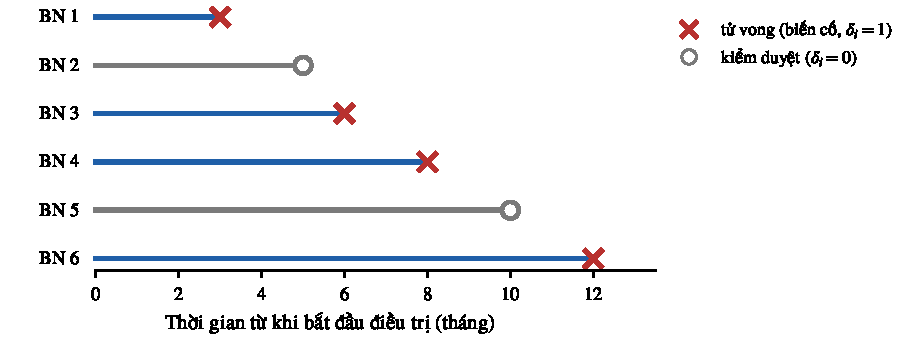
\includegraphics[width=0.85\linewidth]{hinh/lythuyet/h2-1-truc-theo-doi.pdf}
\caption{Trục theo dõi của sáu bệnh nhân. Đường kết thúc bằng biến cố; vòng tròn biểu thị kiểm duyệt.}
\end{figure}


Các nguồn dùng ký hiệu khác nhau, nên báo cáo cố định một bảng đối chiếu để tránh nhầm lẫn khi đối chiếu với tài liệu gốc.
\begin{table}[H]\centering
\caption{Bảng đối chiếu ký hiệu giữa các nguồn.}\label{tab:kyhieu-nguon}
\small
\begin{tabular}{P{4.2cm}P{2.6cm}P{2.7cm}P{3.2cm}}
\toprule
Đại lượng & Chương này & Survival Analysis (Klein 2003) & Bayesian joint ordinal and survival modeling (Armero 2016)\\
\midrule
Thời gian tới biến cố & $T$ & $X$ & $T_i^{*}$ \\
Thời gian kiểm duyệt phải & $C$ & $C_r$ & $C_i$ \\
Thời gian quan sát & $t=\min(T,C)$ & $T=\min(X,C_r)$ & $T_i=\min(T_i^{*},C_i)$\\
Chỉ báo biến cố & $\delta$ & $\delta$ & $\delta_i$\\
Thời điểm vào muộn (cắt cụt trái) & $L$ & $Y_L$ & $a_i$\\
Số người trong tập rủi ro & $R_k$ & $Y_i$ & --\\
Số biến cố tại mốc & $D_k$ & $d_i$ & --\\
Vector hệ số hồi quy PH & $\bm\beta$ & $\bm\beta$ & $\bm\eta$ (phần sống còn)\\
\bottomrule
\end{tabular}
\end{table}
% Lưu ý: \nguon{klein2003} viết AFT là $S(x\mid Z)=S_0[\exp(\bm\theta\tr Z)\,x]$ và hệ số log-thời gian là $\bm\gamma=-\bm\theta$;
% chương này (và \nguon{bartos2022}) dùng $\log T=\bm z\tr\bm\beta+\sigma W$, tức $\bm\beta\equiv\bm\gamma$ của \nguon{klein2003}. Chi tiết ở mục~\ref{sec:phaft}.


%% =====================================================================
\section{Dữ liệu thời gian tới biến cố}
%% =====================================================================

Phân tích sống còn (survival analysis) nghiên cứu khoảng thời gian cho tới khi một biến cố xảy ra.
Biến cố có thể là tử vong, tái phát bệnh, xuất viện, hỏng hóc máy móc hay vỡ nợ. Để định nghĩa
biến phản hồi cần xác định gốc thời gian, thang thời gian và định nghĩa biến cố. Việc chọn gốc
thời gian quyết định câu hỏi nghiên cứu; đơn vị thời gian ảnh hưởng cách diễn giải tham số; còn
định nghĩa biến cố phải phân biệt các biến cố cạnh tranh.
Điều làm phân tích sống còn khác hồi quy thông thường là dữ liệu không đầy đủ: với một số cá
thể, ta không biết thời gian tới biến cố thật sự mà chỉ biết nó dài hơn một mốc. Bỏ các cá thể ấy
hoặc coi mốc đó là thời điểm biến cố đều có thể dẫn tới ước lượng sai.

Ba lựa chọn thiết kế và hai ví dụ thực tế:

\textbf{(a) Gốc thời gian.} Đây là mốc mà tại đó ``đồng hồ'' bắt đầu chạy cho mỗi cá thể: ngày chẩn đoán, ngày ngẫu nhiên hoá,
ngày sinh (khi dùng tuổi làm thang thời gian), lần khám đầu tiên\ldots{} Hai gốc khác nhau trả lời hai câu hỏi khác nhau
(``từ khi chẩn đoán, sống được bao lâu?'' khác ``đến tuổi bao nhiêu thì tử vong?'').
Gốc phải là mốc có thể xác định cho mọi cá thể và xảy ra trước khi cá thể chịu rủi ro.

\textbf{(b) Thang thời gian.} Thời gian lịch, thời gian theo dõi hay tuổi. Khi dùng tuổi, ta thường không quan sát cá thể từ lúc sinh mà chỉ từ tuổi
vào nghiên cứu; đây chính là cắt cụt trái (mục~\ref{sec:cutcut}).

\textbf{(c) Định nghĩa biến cố.} Cần chỉ rõ biến cố nào được tính, và các biến cố khác làm cá thể ``thoát'' khỏi rủi ro thế nào.
Nếu có nhiều biến cố loại trừ nhau (ví dụ tử vong do bệnh khác trước khi chẩn đoán ung thư), đó là \emph{biến cố cạnh tranh}:
\nguon{klein2003, \S2.7} xử lý bằng hazard theo từng nguyên nhân và hàm tần suất tích luỹ.

\medskip
\textbf{Ví dụ 1.} Gốc thời gian là tuổi 50, cận dưới của khoảng tuổi sàng lọc; biến cố là chẩn đoán ung thư vú.
Với phụ nữ không bị chẩn đoán, thời gian kiểm duyệt lấy bằng $\min$(thời điểm tử vong, lần chụp nhũ ảnh cuối $+2{,}5$ năm).
Phụ nữ vào chương trình sau tuổi 50 có thời điểm vào muộn, có thể gây \emph{thiên lệch chọn mẫu theo độ dài} hoặc \emph{cắt cụt trái};
tác giả giải quyết bằng mô hình rủi ro tỉ đối có cắt cụt trái. Đồng thời họ thử coi tử vong là biến cố cạnh tranh và thấy
tần suất tích luỹ ước lượng bằng Kaplan--Meier và bằng hazard theo nguyên nhân gần như trùng nhau, nên dù kiểm duyệt do tử vong
là có thông tin, ảnh hưởng tới ước lượng là nhỏ. \cite{armero2016}

\textbf{Ví dụ 2.} Biến cố là ``tăng ít nhất một bậc Kellgren--Lawrence ở ít nhất một đầu gối giữa hai lần khám''.
Vì chỉ biết biến cố xảy ra \emph{giữa} hai lần khám, về bản chất dữ liệu là kiểm duyệt khoảng (mục~\ref{sec:kiemduyet}). \cite{arbeeva2020}

Không dùng hồi quy thông thường vì hai lý do \cite{arbeeva2020}: (i) thời gian sống thường lệch phải nên không thoả giả định chuẩn; (ii) quan trọng hơn,
thời gian sống thường bị kiểm duyệt, tức không quan sát được ở mọi cá thể.
Với sáu bệnh nhân, trung bình các thời gian quan sát là $44/6\approx 7{,}33$ tháng. Con số này \emph{không} là ước lượng thời gian sống trung bình:
hai giá trị $5$ và $10$ chỉ là cận dưới. Bỏ hai bệnh nhân kiểm duyệt cũng sai vì loại đúng những người sống lâu. Hai cách xử lý sai này được lượng hoá ở mục~\ref{sec:expmle}.

%% =====================================================================
\section{Các hàm cơ bản}
%% =====================================================================

Gọi $T>0$ là thời gian ngẫu nhiên tới biến cố, với mật độ $f(t)$ và hàm phân phối $F(t)=\Prob(T\le t)$.
Hàm sống còn được định nghĩa là
\begin{equation}
S(t)=\Prob(T>t)=1-F(t)=\int_t^\infty f(s)\dd s.
\end{equation}
Đây là xác suất cá thể chưa gặp biến cố tại thời điểm $t$. Hàm bắt đầu ở 1, không tăng theo thời
gian và tiến về 0 nếu cuối cùng mọi cá thể đều gặp biến cố.

Hazard (rủi ro tức thời) được định nghĩa bởi
\begin{equation}
h(t)=\lim_{\Delta t\to0}\frac{\Prob(t\le T<t+\Delta t\mid T\ge t)}{\Delta t}.
\end{equation}
Đây là tốc độ biến cố trong số những cá thể còn sống và đang chịu rủi ro; do đó hazard có đơn vị
nghịch đảo thời gian và không bị chặn trên bởi 1. Với $\Delta t$ nhỏ, xác suất biến cố trong khoảng kế
tiếp xấp xỉ $h(t)\Delta t$.

Từ định nghĩa xác suất có điều kiện suy ra
\begin{equation}\label{eq:hfS}
h(t)=\frac{f(t)}{S(t)}.
\end{equation}
\bs{Thật vậy, $\Prob(t\le T<t+\Delta t\mid T\ge t)=[F(t+\Delta t)-F(t)]/S(t)$; chia cho $\Delta t$ rồi cho $\Delta t\to0$ ta được $F'(t)/S(t)=f(t)/S(t)$.}
Hazard tích luỹ là $H(t)=\int_0^t h(s)\dd s$. Vì $f(t)=-S'(t)$, ta có quan hệ cơ bản
\begin{equation}\label{eq:HS}
H(t)=-\log S(t),\qquad S(t)=\exp\{-H(t)\}.
\end{equation}
\bs{(Từ \eqref{eq:hfS}, $h(t)=-S'(t)/S(t)=-\tfrac{\mathrm d}{\mathrm dt}\log S(t)$; lấy tích phân từ 0 đến $t$ và dùng $S(0)=1$ được \eqref{eq:HS}.)}
Bốn hàm $f$, $S$, $h$ và $H$ xác định lẫn nhau. Mô hình sống còn thường đặc tả hazard trước, rồi suy
ra hàm sống còn và mật độ.


\begin{table}[H]\centering
\caption{Chuyển đổi giữa hàm mật độ, hàm sống còn, hazard và hazard tích lũy.}\label{tab:chuyen-doi-ham}
\small
\begin{tabular}{l@{\hspace{1.2em}}c@{\hspace{1.2em}}c@{\hspace{1.2em}}c@{\hspace{1.2em}}c}
\toprule
Biết $\downarrow$ / Cần $\rightarrow$ & $f(t)$ & $S(t)$ & $h(t)$ & $H(t)$\\
\midrule
$f$ & -- & $\displaystyle\int_t^\infty f$ & $\dfrac{f}{\int_t^\infty f}$ & $-\log\!\int_t^\infty f$\\[8pt]
$S$ & $-S'$ & -- & $-\dfrac{S'}{S}$ & $-\log S$\\[8pt]
$h$ & $h\,e^{-\int_0^t h}$ & $e^{-\int_0^t h}$ & -- & $\int_0^t h$\\[6pt]
$H$ & $H'e^{-H}$ & $e^{-H}$ & $H'$ & --\\
\bottomrule
\end{tabular}
\end{table}
\textbf{Tính chất.} $S$ không tăng, liên tục phải, $S(0)=1$; $H$ không giảm với $H(0)=0$; $h\ge0$ nhưng \emph{không} nhất thiết $\le1$.
Một hàm $h\ge0$ bất kỳ là hazard của một phân phối chính quy (không có khối lượng ở vô cực) khi và chỉ khi $\int_0^\infty h=\infty$.
Điều này cho phép ta tự do \emph{đặc tả hazard} (như Weibull hay mô hình Cox) mà luôn thu được hàm sống còn hợp lệ.

\textbf{Trường hợp rời rạc.} Nếu $T$ nhận các giá trị $t_1<t_2<\cdots$ với hazard rời rạc $h_j=\Prob(T=t_j\mid T\ge t_j)$ thì
$S(t)=\prod_{j:t_j\le t}(1-h_j)$ và $H(t)=\sum_{j:t_j\le t}h_j$; khi đó $H(t)\ne-\log S(t)$ (chỉ xấp xỉ khi $h_j$ nhỏ)
\nguon{klein2003, Ch.\,2}. Công thức tích này chính là cấu trúc của ước lượng Kaplan--Meier ở mục~\ref{sec:km}.

\textbf{Kỳ vọng, trung vị và phần dư kỳ vọng.} Nếu $T\ge0$ thì
\begin{align}
\E[T]&=\int_0^\infty S(t)\dd t,\qquad
t_{p}=\inf\{t:S(t)\le 1-p\}\ \ (\text{trung vị}=t_{0{,}5}),\\
\mathrm{mrl}(t)&=\E[T-t\mid T>t]=\frac{\int_t^\infty S(u)\dd u}{S(t)}.
\end{align}
(Công thức đầu: $\E[T]=\int_0^\infty\!\!\int_0^\infty\ind\{u<T\}\dd u\,\mathrm dF$, đổi thứ tự tích phân.)
Trong dữ liệu có kiểm duyệt, phần đuôi của $S$ thường không quan sát được, nên người ta hay báo cáo \emph{trung vị} hoặc
\emph{thời gian sống trung bình giới hạn} $\int_0^\tau S(t)\dd t$ \cite{klein2003}.


\subsection{Phân phối mũ và Weibull}

Nếu hazard không đổi, $h(t)=\lambda$, thì $H(t)=\lambda t$, $S(t)=e^{-\lambda t}$ và $f(t)=\lambda e^{-\lambda t}$. Trung vị là $\log2/\lambda$.
Với Weibull, đặt $h(t)=\lambda\alpha t^{\alpha-1}$, trong đó $\lambda,\alpha>0$. Khi đó $H(t)=\lambda t^\alpha$ và $S(t)=\exp(-\lambda t^\alpha)$. Tham
số $\alpha<1$ cho hazard giảm, $\alpha=1$ cho hazard hằng và $\alpha>1$ cho hazard tăng.

% \begin{figure}[ht]\centering
% \begin{tikzpicture}
% \begin{axis}[width=7.5cm,height=5cm,axis lines=left,xlabel={$t$},ylabel={$h(t)$},
%  xmin=0,xmax=3,ymin=0,ymax=3.2,ticks=none,domain=0.05:3,samples=60,
%  legend pos=north east,legend style={font=\small,draw=none}]
% \addplot[thick,blue!70!black]{1.5*0.8*x^0.8}; \addlegendentry{tăng ($\alpha>1$)}
% \addplot[thick,black]{1.0+0*x}; \addlegendentry{hằng ($\alpha=1$)}
% \addplot[thick,red!70!black]{0.8*0.6*x^(-0.4)}; \addlegendentry{giảm ($\alpha<1$)}
% \end{axis}
% \end{tikzpicture}
% \caption{Ba dạng hazard Weibull theo tham số hình dạng. (Minh họa định tính; đường tăng vẽ với $\alpha=1{,}8$, đường giảm với $\alpha=0{,}6$, hằng số $\lambda$ chọn để các đường dễ phân biệt.)}
% \end{figure}

\begin{figure}[H]\centering
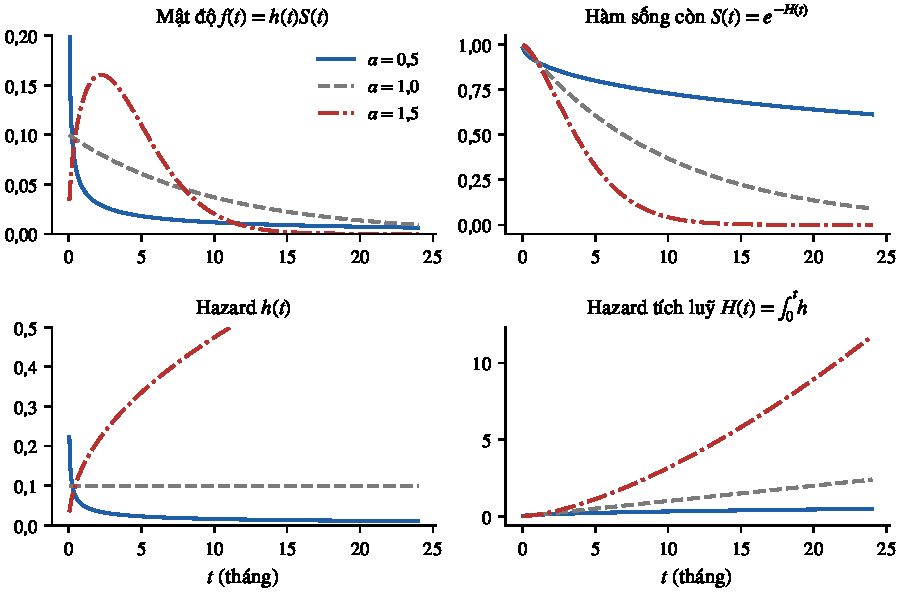
\includegraphics[width=0.85\linewidth]{hinh/lythuyet/h2-3-bon-ham.pdf}
\caption{Bốn hàm của các phân phối Weibull.}
\end{figure}

% \begin{chinhsua}[Hình 2]
% Trong bản gốc Hình~2 là hình vẽ TikZ không có nhãn trục số; tôi dựng lại một hình tương đương chỉ để tài liệu biên dịch được. Nếu bạn có sẵn mã TikZ gốc, hãy giữ mã của bạn.
% \end{chinhsua}

Công thức đầy đủ cho mũ/Weibull và đối chiếu với dữ liệu sáu bệnh nhân
\textbf{Weibull.} Với $S(t)=\exp(-\lambda t^\alpha)$:
\begin{align}
\E[T]&=\int_0^\infty e^{-\lambda t^\alpha}\dd t=\lambda^{-1/\alpha}\,\Gamma\!\left(1+\tfrac1\alpha\right),&
t_{0{,}5}&=\left(\frac{\log2}{\lambda}\right)^{1/\alpha},\\
h'(t)&=\lambda\alpha(\alpha-1)t^{\alpha-2}\ \Rightarrow\ \text{dấu của }h'\text{ là dấu của }\alpha-1.&&
\end{align}
Trường hợp mũ ($\alpha=1$) có tính \emph{không nhớ}: $\mathrm{mrl}(t)=1/\lambda$ với mọi $t$.
Khi $\alpha\ne1$ hazard đơn điệu; Weibull \emph{không} mô tả được hazard hình chuông (log-logistic, log-normal làm được, xem Bảng~\ref{tab:phanphoi}).

\textbf{Ví dụ với sáu bệnh nhân.} Dùng $\hat\lambda=4/44\approx0{,}0909$ (mục~\ref{sec:expmle}), mô hình mũ cho
$\hat S(3)\approx0{,}761$, $\hat S(6)\approx0{,}580$, $\hat S(8)\approx0{,}483$, so với Kaplan--Meier $0{,}833$, $0{,}625$, $0{,}417$ (Bảng~\ref{tab:km}).
Hai đường cùng cho trung vị quanh $7{,}6$--$8$ tháng nhưng khác dạng: dữ liệu có xu hướng hazard tăng (các biến cố dồn về cuối),
điều mà mô hình mũ hazard hằng không bắt được. Mô hình Weibull khớp bằng hợp lý cực đại trên cùng dữ liệu cho $\hat\alpha\approx2{,}53$ (hazard tăng) và
$\hat\lambda\approx3{,}27\times10^{-3}$; log-hợp-lý $-11{,}82$ so với $-13{,}59$ của mô hình mũ, thống kê tỉ số hợp lý $\approx3{,}55$ (1 bậc tự do; $p\approx0{,}06$). Với $n=6$ đây chỉ là minh hoạ về cách đọc,
không phải bằng chứng.


%% =====================================================================
\section{Kiểm duyệt}\label{sec:kiemduyet}
%% =====================================================================

Kiểm duyệt nghĩa là ta không quan sát được biến cố trong thời gian theo dõi, nhưng vẫn biết cá
thể chưa gặp biến cố tới một mốc. Trong ví dụ sáu bệnh nhân, bệnh nhân 2 và 5 bị kiểm duyệt;
ta biết họ sống ít nhất 5 và 10 tháng.

Gọi $T_i$ là thời gian tới biến cố và $C_i$ là thời gian kiểm duyệt. Ta quan sát
\begin{equation}
t_i=\min(T_i,C_i),\qquad\delta_i=\ind\{T_i\le C_i\}.
\end{equation}
Kiểm duyệt phải cho biết $T_i>C_i$; kiểm duyệt trái cho biết $T_i<C_i$; kiểm duyệt khoảng cho biết
$t_i^L<T_i\le t_i^R$.

\begin{table}[H]\centering
\caption{Đóng góp vào hàm hợp lý theo thông tin quan sát.}
\begin{tabular}{llc}
\toprule
Loại & Điều biết được & Đóng góp\\
\midrule
Biến cố tại $t_i$ & $T_i=t_i$ & $f(t_i)=h(t_i)S(t_i)$\\
Kiểm duyệt phải & $T_i>C_i$ & $S(C_i)$\\
Kiểm duyệt trái & $T_i<C_i$ & $1-S(C_i)$\\
Kiểm duyệt khoảng & $t_i^L<T_i\le t_i^R$ & $S(t_i^L)-S(t_i^R)$\\
\bottomrule
\end{tabular}
\end{table}

Các đóng góp trên dựa vào giả định kiểm duyệt độc lập có điều kiện theo hiệp biến: $T\indep C\mid z$.
Sau khi đã biết các hiệp biến, thời điểm bị kiểm duyệt không cung cấp thêm thông tin về rủi ro
biến cố. Giả định này khác với việc các tham số của mô hình kiểm duyệt không liên quan đến tham số sống còn; điều kiện thứ hai cho phép bỏ thừa số kiểm duyệt khỏi hàm hợp lý.

\begin{figure}[H]\centering
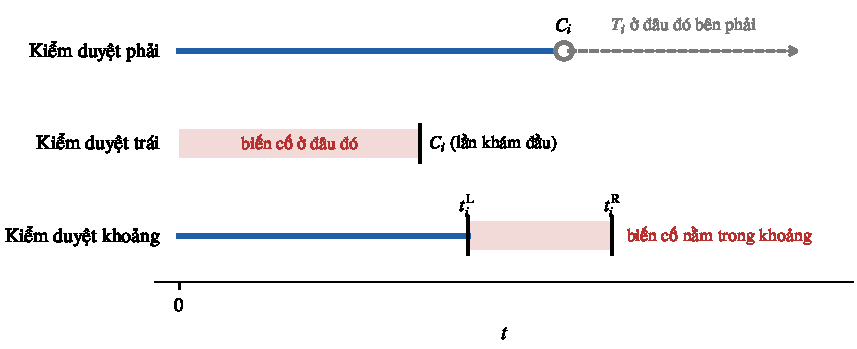
\includegraphics[width=0.85\linewidth]{hinh/lythuyet/h2-6-ba-loai-kiem-duyet.pdf}
\caption{Ba loại kiểm duyệt; vùng tô màu là khoảng thời gian có thể xảy ra biến cố.}
\end{figure}

Cần phân biệt bốn cơ chế kiểm duyệt phải; chúng đều dẫn tới cùng dạng hợp lý nhưng khác ở chỗ thời điểm kiểm duyệt do ai quyết định \cite{klein2003}:

\begin{center}\small
\begin{table}[H]\centering
\caption{Các cơ chế kiểm duyệt phải}
\begin{tabular}{P{2.8cm}P{5.2cm}P{4.4cm}}
\toprule
Cơ chế & Mô tả & Ví dụ\\
\midrule
Loại I & Mọi cá thể bị kiểm duyệt tại một mốc cố định $C$ & Thử nghiệm dừng sau 12 tháng\\
Loại II & Dừng khi đã quan sát $r$ biến cố trong $n$ cá thể & Thử nghiệm độ bền linh kiện\\
Ngẫu nhiên & Mỗi cá thể có $C_i$ riêng, ngẫu nhiên, độc lập với $T_i$ & Vào nghiên cứu lệch thời điểm, rút lui\\
Luỹ tiến & Rút cá thể ra ở nhiều thời điểm ``hy sinh'' định trước & Thí nghiệm trên chuột\\
\bottomrule
\end{tabular}
\end{table}
\end{center}
\newpage
% Trong ví dụ sáu bệnh nhân, bệnh nhân 5 là kiểm duyệt do \emph{hết nghiên cứu} (hành chính), bệnh nhân 2 là kiểm duyệt do \emph{mất liên lạc}.
% Hai trường hợp này khác nhau về mức độ đáng ngờ của giả định độc lập.


% Chứng minh: vì sao kiểm duyệt độc lập cho phép bỏ thừa số kiểm duyệt
% Giả sử $T$ có mật độ $f$, hàm sống còn $S$; $C$ độc lập với $T$, có mật độ $g$ và hàm sống còn $G$. Với $t=\min(T,C)$ và $\delta=\ind\{T\le C\}$:
% \begin{align*}
% \Prob(t\in\dd u,\delta=1)&=\Prob(T\in\dd u,\ C\ge u)=f(u)\,G(u)\dd u,\\
% \Prob(t\in\dd u,\delta=0)&=\Prob(C\in\dd u,\ T>u)=g(u)\,S(u)\dd u.
% \end{align*}
% Hợp lại $\Prob(t,\delta)=[f(t)G(t)]^{\delta}\,[g(t)S(t)]^{1-\delta}$, nên
% \[
% L=\underbrace{\prod_{i=1}^n G(t_i)^{\delta_i}g(t_i)^{1-\delta_i}}_{\text{chỉ chứa tham số kiểm duyệt}}\ \times\ \prod_{i=1}^n f(t_i)^{\delta_i}S(t_i)^{1-\delta_i}.
% \]


% \textbf{Khi giả định có thể sai (kiểm duyệt có thông tin).} Nếu bệnh nhân 2 ``mất liên lạc'' vì đang chuyển nặng, phần thông tin về $T_2$ nằm trong cơ chế kiểm duyệt.
% Một cách đánh giá nhạy cảm đơn giản: với mô hình mũ, nếu hai người bị kiểm duyệt thực ra \emph{đều chết ngay tại mốc kiểm duyệt} thì $\hat\lambda=6/44\approx0{,}136$;
% nếu họ \emph{đều sống đến tháng 12} (cận cuối cửa sổ quan sát) thì $\hat\lambda=4/(3+12+6+8+12+12)=4/53\approx0{,}075$.
% Ước lượng $0{,}091$ nằm giữa hai kịch bản cực đoan $[0{,}075;\,0{,}136]$, cho biết độ rộng của sai lệch nếu giả định độc lập bị vi phạm. (Kịch bản trên chỉ là minh hoạ do tôi đặt, không lấy từ nguồn.)



% \textbf{Kiểm duyệt trái} khi biến cố đã xảy ra \emph{trước} lần quan sát đầu (ví dụ khám lần đầu đã thấy bệnh, không biết khởi phát khi nào), đóng góp $1-S(C_i)=F(C_i)$.
% \textbf{Kiểm duyệt khoảng} khi theo dõi bằng các lần khám định kỳ: lần khám thứ $j-1$ âm tính, lần $j$ dương tính thì $T\in(t_{j-1},t_j]$, đóng góp $S(t_{j-1})-S(t_j)$
% \nguon{klein2003, \S3.3}. Kiểm duyệt phải là trường hợp $t^R=\infty$, kiểm duyệt trái là $t^L=0$.
% Dữ liệu của \nguon{arbeeva20} (biến cố phát hiện ở các lần chụp X-quang cách nhau nhiều năm) và các thiết kế dựa trên khám định kỳ nói chung là kiểm duyệt khoảng.
% Phần \nguon{bartos2022} ghi chú rằng khung Bayes tham số \emph{dễ mở rộng} sang kiểm duyệt trái và khoảng, chỉ cần thay thừa số hợp lý theo Bảng~2.
% \end{bosung}

%% =====================================================================
\section{Cắt cụt trái và vào trễ}\label{sec:cutcut}
%% =====================================================================

Khác với kiểm duyệt, cắt cụt quyết định cá thể nào được vào mẫu. Với cắt cụt trái (vào trễ), cá
thể chỉ được quan sát từ thời điểm $L_i>0$; chỉ người còn sống tới thời điểm đó mới có mặt trong
dữ liệu. Ví dụ, nghiên cứu tuổi thọ từ dữ liệu viện dưỡng lão có thiên lệch chọn mẫu vì người tham
gia đã phải sống tới tuổi vào viện.

Với biến cố tại $t_i\ge L_i$, mật độ có điều kiện là $f(t_i)/S(L_i)$. Với kiểm duyệt phải tại $t_i$, xác suất có
điều kiện là $S(t_i)/S(L_i)$. Do đó
\begin{equation}\label{eq:trunc}
\frac{f(t_i)}{S(L_i)}\ \ (\text{biến cố}),\qquad\frac{S(t_i)}{S(L_i)}\ \ (\text{kiểm duyệt phải}).
\end{equation}
Bỏ mẫu số tương đương với tính nhầm thời gian trước điểm vào như thời gian chịu rủi ro, có thể
gây thiên lệch. Kiểm duyệt che một phần quỹ đạo của cá thể đã vào mẫu; cắt cụt quyết định cá
thể có được vào mẫu hay không.

\begin{figure}[H]\centering
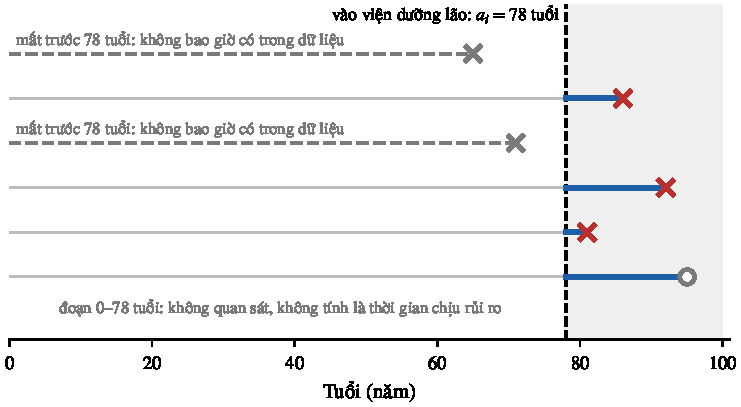
\includegraphics[width=0.85\linewidth]{hinh/lythuyet/h2-7-cat-cut-trai.pdf}

\caption{Minh họa cắt cụt trái và vào trễ.}
\end{figure}

\begin{table}[H]\centering
\caption{Phân biệt cắt cụt và kiểm duyệt; các loại cắt cụt}
\begin{center}\small
\begin{tabular}{P{3.2cm}P{5.1cm}P{5.0cm}}
\toprule
 & Kiểm duyệt & Cắt cụt\\
\midrule
Cá thể có trong mẫu? & Có, luôn được ghi nhận & Chỉ khi biến cố rơi vào cửa sổ quan sát\\
Thông tin mất & Một phần (biết $T>C$, hoặc $T\in$ khoảng) & Toàn bộ cá thể ngoài cửa sổ không để lại dấu vết\\
Cách xử lý & Thay mật độ bằng $S$, $1-S$, $S(L)-S(R)$ & Dùng xác suất \emph{có điều kiện} theo cửa sổ\\
\bottomrule
\end{tabular}
\end{center}
\end{table}

\nguon{klein2003, \S3.4}: chỉ quan sát cá thể có $T$ nằm trong cửa sổ $(Y_L,Y_R)$.
\emph{Cắt cụt trái} ($Y_R=\infty$): quan sát $T$ khi và chỉ khi $T>Y_L$; ví dụ khách của viện dưỡng lão Channing House phải sống đủ tuổi để vào viện
(Ex.~3.7), hoặc nghiên cứu ``thời gian từ ghép tủy đến tử vong'' chỉ trên những người đã hồi phục tiểu cầu (Ex.~9.5; lúc đó thời điểm hồi phục là thời điểm vào muộn).
\emph{Cắt cụt phải} ($Y_L=0$): chỉ quan sát $T\le Y_R$, điển hình là phân tích sổ đăng ký chỉ chứa ca đã mắc bệnh tính đến ngày lấy mẫu (Ex.~3.8, AIDS do truyền máu).
Đóng góp hợp lý \nguon{klein2003, \S3.5}:
\begin{center}\small
\begin{tabular}{lc}
\toprule
Cắt cụt trái & $f(t)/S(Y_L)$\\
Cắt cụt phải & $f(t)/[1-S(Y_R)]$\\
Cắt cụt khoảng & $f(t)/[S(Y_L)-S(Y_R)]$\\
\bottomrule
\end{tabular}
\end{center}
Hệ quả: suy luận với dữ liệu bị cắt cụt luôn là suy luận \emph{có điều kiện}.


\begin{bosung}[Vào trễ trong thực tế: Armero16 và Channing House; điều kiện hợp lệ]
\textbf{Armero16, \S3.} Phụ nữ vào chương trình sàng lọc ở tuổi $a_i>50$ nên hazard của $T_i^{*}$ được định nghĩa bằng $0$ trước $a_i$:
\[
h_i(t)=h_0(t)\exp\{\bm x_i\tr\bm\eta+\alpha m_i(t)\},\ \ t>a_i,\qquad h_i(t)=0\ \text{trong trường hợp còn lại,}
\]
và tác giả nhấn mạnh rằng hợp lý của dữ liệu cắt cụt trái chứa các xác suất có điều kiện ``người đó còn sống từ tuổi 50 đến $a_i$''
nên \emph{làm tăng độ phức tạp tính toán}. Họ chọn $h_0$ Weibull và gọi cắt cụt trái là ``cơ chế hiệu chỉnh thiên lệch vào trễ''.

\textbf{Điều kiện hợp lệ} \nguon{klein2003, Ch.\,9 \S9.4}. Việc điều kiện hoá theo $S(L_i)$ chỉ đúng khi thời điểm vào $L_i$ \emph{độc lập với $T_i$ cho trước hiệp biến}.
Tập rủi ro trở thành $R(t)=\{j: L_j<t\le t_j\}$ và các phương pháp Chương~8 dùng nguyên văn với tập rủi ro này.
\emph{Lưu ý thực hành} (Practical note~1, \S9.4): nếu dùng tuổi làm điểm cắt cụt thì không cần đưa tuổi vào mô hình làm hiệp biến thêm lần nữa; ``tuổi'' thường bị đưa nhầm vào vai hiệp biến trong khi đúng vai là điểm cắt cụt.

\textbf{Ước lượng.} Với $Y_i=\#\{j:L_j<t_i\le t_j\}$ thay cho số ở rủi ro thông thường, mọi công thức của \S4.2--4.4 dùng được, nhưng
ước lượng tích-giới-hạn lúc này ước lượng $\Prob(X>t\mid X\ge a)=S(t)/S(a)$ chứ không phải $S(t)$ \nguon{klein2003, \S4.6}.
Cẩn trọng khi tập rủi ro nhỏ ở các mốc sớm (ví dụ chỉ 1--2 người): chỉ cần $Y_i=d_i$ tại một mốc thì $\hat S$ về 0 ngay dù về sau còn nhiều người sống, nên người ta ước lượng điều kiện từ một mốc đủ lớn trở đi (Channing House, Ex.~4.3).

\textbf{Thiên lệch theo độ dài (length-biased sampling).} \nguon{armero16} chỉ nhắc rằng vào trễ ``có thể gây thiên lệch theo độ dài hoặc cắt cụt trái''.
Phần sau là kiến thức bổ sung \emph{ngoài} các tài liệu đã cung cấp, nên cần kiểm chứng trước khi trích dẫn: khi lấy mẫu một nhóm \emph{đang mắc} (prevalent cohort) từ một quá trình khởi phát ổn định theo thời gian,
xác suất một cá thể được chọn tỉ lệ thuận với độ dài thời gian sống của nó, nên mật độ quan sát được là $f_{LB}(t)=t f(t)/\E[T]$, lệch về giá trị lớn.
Đây là trường hợp đặc biệt của cắt cụt trái trong đó thời điểm vào có phân phối đều ngược thời gian; hợp lý có điều kiện theo $L_i$ (\eqref{eq:trunc}) vẫn hợp lệ nhưng không khai thác hết thông tin về tính ổn định của quá trình khởi phát.
\end{bosung}

\begin{vidu}[Ví dụ sáu bệnh nhân: giả định thêm thời điểm vào muộn (số liệu giả định)]
\textit{Phần dưới do tôi thêm; thời điểm vào $L_i$ là giả định để minh hoạ, không có trong \texttt{main.pdf}.} Giữ $t_i,\delta_i$ của Bảng~1 và đặt
$L=(0,\,0,\,2,\,4,\,0,\,7)$: bệnh nhân 3, 4, 6 vào lần lượt ở tháng 2, 4, 7 (mỗi người đều còn sống tới thời điểm vào của mình).
\begin{itemize}[leftmargin=1.4em,itemsep=1pt]
\item \textbf{Mô hình mũ.} Theo \eqref{eq:trunc}, $\ell(\lambda)=D\log\lambda-\lambda\sum_i(t_i-L_i)$ và $\hat\lambda=D/\sum_i(t_i-L_i)=4/(44-13)=4/31\approx0{,}129$ mỗi tháng.
Nếu bỏ qua $L_i$ ta được $4/44\approx0{,}091$, \emph{thấp hơn} vì tính nhầm $13$ tháng-người ``không ai theo dõi'' vào mẫu số. Trung vị tương ứng: $\log2/0{,}129\approx5{,}4$ tháng thay vì $7{,}6$.
\item \textbf{Tích-giới-hạn.} Tập rủi ro lúc này là $\{L_j<t\le t_j\}$:
\begin{center}\small
\begin{tabular}{cccc}
\toprule
$t_{(k)}$ & $Y_k$ & $d_k$ & $\hat S(t_{(k)})$ (có điều kiện theo vào trễ)\\
\midrule
3 & 4 (BN 1,2,3,5) & 1 & $3/4=0{,}750$\\
6 & 3 (BN 3,4,5) & 1 & $0{,}750\times 2/3=0{,}500$\\
8 & 3 (BN 4,5,6) & 1 & $0{,}500\times 2/3=0{,}333$\\
12 & 1 (BN 6) & 1 & $0$\\
\bottomrule
\end{tabular}
\end{center}
Kết quả thấp hơn Kaplan--Meier gốc ($0{,}833;0{,}625;0{,}417$): bỏ qua cắt cụt làm \emph{thổi phồng} sống còn, vì coi người chưa vào mẫu cũng đã ở trong tập rủi ro.
\end{itemize}
\end{vidu}

%% =====================================================================
\section{Hàm hợp lý có kiểm duyệt và cắt cụt}
%% =====================================================================

Với các quan sát độc lập $(t_i,\delta_i,L_i)$, trong đó $L_i=0$ nếu không vào trễ, hàm hợp lý là
\begin{equation}\label{eq:lik}
L(\vartheta)=\prod_{i=1}^n\frac{h(t_i)^{\delta_i}S(t_i)}{S(L_i)}.
\end{equation}
Lấy logarit và dùng $\log S=-H$:
\begin{equation}\label{eq:loglik}
\ell(\vartheta)=\sum_{i=1}^n\{\delta_i\log h(t_i)-[H(t_i)-H(L_i)]\}.
\end{equation}
Mỗi biến cố đóng góp log-hazard tại thời điểm xảy ra; mọi cá thể đóng góp phần hazard tích luỹ
trong khoảng thời gian được quan sát.

\begin{bosung}[Dạng tổng quát khi trộn nhiều loại thông tin; dạng quá trình đếm]
Gộp các thông tin của Bảng~2 và cắt cụt trái \eqref{eq:trunc}, với $\mathcal D,\mathcal R,\mathcal L,\mathcal I$ lần lượt là tập các quan sát biến cố, kiểm duyệt phải, kiểm duyệt trái và kiểm duyệt khoảng
\nguon{klein2003, (3.5.1)--(3.5.2)}:
\begin{equation}
L(\vartheta)\ \propto\ \prod_{i\in\mathcal D}\frac{f(t_i)}{S(L_i)}\prod_{i\in\mathcal R}\frac{S(t_i)}{S(L_i)}
\prod_{i\in\mathcal L}\frac{S(L_i)-S(t_i)}{S(L_i)}\prod_{i\in\mathcal I}\frac{S(t_i^L)-S(t_i^R)}{S(L_i)}.
\end{equation}
(Với kiểm duyệt trái trên cá thể vào trễ, xác suất có điều kiện là $\Prob(T<c\mid T>L)=[S(L)-S(c)]/S(L)$, không còn là $1-S(c)$. Đây là hệ quả trực tiếp của điều kiện hoá; tôi suy ra, không trích nguyên văn từ tài liệu.)
Nếu mỗi cá thể có phân phối riêng (hồi quy) thì thay $f,S$ bằng $f_i,S_i$ \nguon{klein2003, (3.5.2)}.

\textbf{Dạng quá trình đếm.} Đặt $N_i(t)=\ind\{t_i\le t,\ \delta_i=1\}$ và chỉ báo rủi ro $Y_i(t)=\ind\{L_i<t\le t_i\}$. Khi đó \eqref{eq:loglik} viết lại
\[
\ell(\vartheta)=\sum_{i=1}^n\left\{\int_0^\infty\log h_i(s)\dd N_i(s)-\int_0^\infty Y_i(s)\,h_i(s)\dd s\right\}.
\]
Dạng này cho thấy: (i) cắt cụt trái và kiểm duyệt phải chỉ đơn giản \emph{đổi cửa sổ} $Y_i(s)$ mà cá thể chịu rủi ro; (ii) log-hợp-lý giống log-hợp-lý của một quá trình Poisson với cường độ $Y_i(s)h_i(s)$
\nguon{klein2003, \S3.6}. Chính điều (ii) là cơ sở của cách ``chia khoảng'' ở Cox có biến phụ thuộc thời gian (mục~\ref{sec:tvc}) và cho phép khớp mô hình sống còn bằng hồi quy Poisson có offset $\log(\text{thời gian})$
(kiến thức thống kê chung, không lấy từ các tài liệu đã cung cấp).
\end{bosung}

\subsection{Ước lượng hazard mũ}\label{sec:expmle}

Với mô hình mũ $h(t)=\lambda$, $H(t)=\lambda t$ và không vào trễ,
\[
\ell(\lambda)=D\log\lambda-\lambda\sum_i t_i,\qquad D=\sum_i\delta_i.
\]
Cho đạo hàm bằng 0 thu được
\begin{equation}\label{eq:lamhat}
\hat\lambda=\frac{D}{\sum_i t_i}.
\end{equation}
Với sáu bệnh nhân, $\hat\lambda=4/44\approx0{,}091$ mỗi tháng; trung vị ước lượng là $\log(2)/\hat\lambda\approx7{,}6$ tháng. Bỏ
hai bệnh nhân kiểm duyệt cho $4/29\approx0{,}138$; coi kiểm duyệt là tử vong cho $6/44\approx0{,}136$. Cả hai
cách đều làm sai lệch ước lượng vì bỏ hoặc bịa ra thông tin biến cố.

\begin{figure}[ht]\centering
\hinhlt{h2-9-loglik}
\caption{Log-hợp-lý theo các cách xử lý kiểm duyệt.}
\end{figure}

\begin{figure}[ht]\centering
\hinhlt{h2-8-mo-phong-kiem-duyet}
\caption{Minh họa mô phỏng so sánh các cách xử lý kiểm duyệt và cắt cụt.}
\end{figure}

\begin{bosung}[Suy luận đầy đủ cho mô hình mũ và Weibull]
\textbf{Phương sai và khoảng tin cậy.} $\ell''(\lambda)=-D/\lambda^2$ nên thông tin quan sát là $D/\hat\lambda^2$ và $\widehat{\Var}(\hat\lambda)=\hat\lambda^2/D$, tức $\mathrm{se}(\hat\lambda)=\hat\lambda/\sqrt D$.
Độ chính xác phụ thuộc vào số \emph{biến cố} $D$, không phải $n$. Khoảng Wald trên thang log: $\hat\lambda\exp\{\pm1{,}96/\sqrt D\}$.
Với sáu bệnh nhân: $\mathrm{se}=0{,}091/2=0{,}0455$; khoảng $95\%$ là $[0{,}034;\,0{,}242]$ mỗi tháng, tương ứng trung vị từ $2{,}9$ đến $20{,}3$ tháng, rất rộng, đúng như ta kỳ vọng từ $D=4$.
Giá trị cực đại của log-hợp-lý: $\ell(\hat\lambda)=D\log(D/T)-D=4\log(4/44)-4\approx-13{,}59$ (với $T=\sum t_i$).

\textbf{Có cắt cụt trái.} \eqref{eq:loglik} cho $\hat\lambda=D/\sum_i(t_i-L_i)$ (xem ví dụ giả định ở mục~\ref{sec:cutcut}).

\textbf{Weibull: không có nghiệm đóng.} $\ell(\lambda,\alpha)=D\log(\lambda\alpha)+(\alpha-1)\sum_i\delta_i\log t_i-\lambda\sum_i t_i^\alpha$.
Cho $\partial\ell/\partial\lambda=0$ được $\hat\lambda(\alpha)=D/\sum_i t_i^\alpha$; thế vào, $\hat\alpha$ là nghiệm của
\[
\frac D\alpha+\sum_i\delta_i\log t_i-D\,\frac{\sum_i t_i^\alpha\log t_i}{\sum_i t_i^\alpha}=0,
\]
giải bằng phương pháp số. Với sáu bệnh nhân: $\hat\alpha\approx2{,}53$, $\hat\lambda\approx3{,}27\times10^{-3}$. Trong tham số hoá log-tuyến tính của \nguon{klein2003, (12.2.6)}:
$\sigma=1/\alpha$, $\mu=-\log\lambda/\alpha$, tức $\hat\sigma\approx0{,}40$, $\hat\mu\approx2{,}27$.

\textbf{Khung Bayes.} \nguon{bartos2022, (1)--(3)}: hợp lý $p(\text{data}\mid\theta)=\prod_i h(t_i\mid x_i,\theta)^{\ind(c_i=1)}S(t_i\mid x_i,\theta)$ (đúng là \eqref{eq:lik} khi $L_i=0$),
hậu nghiệm $p(\theta\mid\text{data})\propto p(\text{data}\mid\theta)p(\theta)$ và hợp lý biên $p(\text{data})=\int p(\text{data}\mid\theta)p(\theta)\dd\theta$ dùng cho so sánh mô hình bằng nhân tử Bayes.
Mô hình mũ có tiên nghiệm liên hợp: nếu $\lambda\sim\mathrm{Gamma}(a,b)$ (tham số tốc độ) thì $\lambda\mid\text{data}\sim\mathrm{Gamma}(a+D,\,b+\sum_i t_i)$. Với $a=1$, $b=10$ (trung bình tiên nghiệm $0{,}1$) ta được
$\mathrm{Gamma}(5,54)$: trung bình hậu nghiệm $0{,}093$, khoảng tin cậy $95\%$ (khoảng tin cậy hậu nghiệm) $[0{,}030;\,0{,}190]$. (Số tiên nghiệm do tôi chọn, chỉ để minh hoạ.)

\textbf{Liên hệ với INLA.} Trong khuôn khổ mô hình Gauss tiềm ẩn, \eqref{eq:lik} đóng vai \emph{hợp lý quan sát} $p(y_i\mid\eta_i,\theta)$ với $\eta_i$ là bộ dự báo tuyến tính (ví dụ $\log h$ trong mô hình PH);
điều kiện cần là các quan sát độc lập có điều kiện khi cho trường tiềm ẩn, điều \eqref{eq:lik} thoả vì nó là tích theo $i$. (Đoạn này dựa trên hiểu biết chung về INLA; \nguon{rustand2026} và SurvINLA chưa được cung cấp nên tôi chưa đối chiếu được. Xem Phụ lục B.)
\end{bosung}

%% =====================================================================
\section{Mô hình hồi quy: PH so với AFT}\label{sec:phaft}
%% =====================================================================

Mô hình hazard tỉ lệ (PH) là
\begin{equation}\label{eq:ph}
h(t\mid\bm z)=h_0(t)\exp(\bm z\tr\bm\beta),
\end{equation}
trong đó $h_0(t)$ là hazard nền. Với hai cá thể, tỉ số hazard không phụ thuộc thời gian; nếu khác
nhau một đơn vị ở hiệp biến thứ $p$, hazard ratio là $e^{\beta_p}$. Ví dụ $\hat\beta=-0{,}35$ cho $\mathrm{HR}\approx0{,}70$, tức
hazard tức thời thấp hơn 30\%, chứ không đồng nghĩa xác suất tử vong thấp hơn 30\%.

Mô hình thời gian thất bại gia tốc (AFT) được viết
\begin{equation}\label{eq:aft}
\log T=\bm z\tr\bm\beta+\sigma_W W,\qquad W\sim f_W.
\end{equation}
Hệ số $e^{\beta_p}$ là tỉ số thời gian: nó co giãn các phân vị thời gian sống. PH mô tả tác động lên hazard
tức thời; AFT mô tả tác động lên thời gian sống. Weibull là trường hợp đặc biệt có thể biểu diễn
dưới cả hai dạng, với quy đổi
\begin{equation}\label{eq:conv}
\bm\beta^{\mathrm{AFT}}=-\bm\beta^{\mathrm{PH}}/\alpha.
\end{equation}

\begin{figure}[ht]\centering
\hinhlt{h2-10-ph-aft}
\caption{So sánh cách diễn giải PH và AFT.}
\end{figure}

\begin{figure}[ht]\centering
\hinhlt{h2-11-vi-pham-ph}
\caption{Minh họa các đường hazard giao nhau khi giả định PH không phù hợp.}
\end{figure}

\begin{chinhsua}[Phương trình \eqref{eq:aft}]
Bản gốc viết $\log T=\bm z\tr\bm\beta+\sigma_WW$ không có hằng số. Nếu $\bm z$ có cột 1 (hệ số chặn) thì đúng; nếu không, cần thêm $\mu$:
$\log T=\mu+\bm z\tr\bm\beta+\sigma W$, như \nguon{klein2003, (12.1.3)}. Tôi giữ nguyên bản gốc và nêu ở đây để bạn thống nhất ký hiệu với phần Weibull bên dưới. Ngoài ra, ký hiệu $\sigma_W$ trong bản gốc tôi đọc là độ co giãn của sai số $W$ (cùng nghĩa với $\sigma$ của \nguon{klein2003}).
\end{chinhsua}

\begin{bosung}[Suy dẫn chi tiết: PH, AFT và phép quy đổi Weibull]
\textbf{PH.} Từ \eqref{eq:ph}: $H(t\mid\bm z)=e^{\bm z\tr\bm\beta}H_0(t)$ và
\begin{equation}
S(t\mid\bm z)=S_0(t)^{\exp(\bm z\tr\bm\beta)}.
\end{equation}
Hiệp biến chỉ \emph{nâng luỹ thừa} hàm sống còn nền; hai đường sống còn không bao giờ cắt nhau. Hệ số $\beta_p$ không nói gì trực tiếp về xác suất sống tại một thời điểm.

\textbf{AFT.} Đặt $S_0$ là hàm sống còn của $e^{\mu+\sigma W}$. Khi đó \nguon{klein2003, (12.1.1)--(12.1.2)}
\begin{equation}
S(t\mid\bm z)=S_0\!\left(t\,e^{-\bm z\tr\bm\gamma}\right),\qquad h(t\mid\bm z)=e^{-\bm z\tr\bm\gamma}\,h_0\!\left(t\,e^{-\bm z\tr\bm\gamma}\right),
\end{equation}
với $\bm\gamma$ là hệ số của $\bm z$ trong $\log T$ (ở bản gốc là $\bm\beta$). Mọi phân vị nhân với $e^{\bm z\tr\bm\gamma}$; trung vị của nhóm có hiệp biến $\bm z$ bằng trung vị nền nhân $e^{\bm z\tr\bm\gamma}$.
\textbf{Cảnh báo ký hiệu:} \nguon{klein2003} định nghĩa ``acceleration factor'' là $\exp(\bm\theta\tr Z)$ với $\bm\theta=-\bm\gamma$ (nên giá trị $>1$ nghĩa là thời gian \emph{rút ngắn}),
còn \nguon{bartos2022} dùng $\mathrm{AF}>1$ nghĩa là sống \emph{lâu hơn} (cùng chiều với $e^{\gamma}$). Chương này gọi $e^{\beta}$ là \emph{tỉ số thời gian} để tránh nhầm.

\textbf{Weibull thuộc cả hai họ.} Với $h(t\mid\bm z)=\lambda\alpha t^{\alpha-1}e^{\bm z\tr\bm\beta^{\mathrm{PH}}}$, $S(t\mid\bm z)=\exp\{-\lambda e^{\bm z\tr\bm\beta^{\mathrm{PH}}}t^{\alpha}\}$. Với $Y=\log T$:
\[
\Prob(Y>y\mid\bm z)=\exp\{-\lambda\,e^{\bm z\tr\bm\beta^{\mathrm{PH}}}e^{\alpha y}\}=\exp\Big\{-e^{\alpha(y-\mu-\bm z\tr\bm\gamma)}\Big\}=S_W\!\Big(\frac{y-\mu-\bm z\tr\bm\gamma}{\sigma}\Big),
\]
trong đó $S_W(w)=\exp(-e^{w})$ là hàm sống còn của phân phối cực trị chuẩn, với $\sigma=1/\alpha$, $\mu=-\log\lambda/\alpha$ và, so khớp số mũ, $\bm\gamma=-\bm\beta^{\mathrm{PH}}/\alpha$, đó chính là \eqref{eq:conv}.
Ví dụ: $\beta^{\mathrm{PH}}=-0{,}35$ và $\alpha=1{,}5$ cho $\gamma=0{,}233$, tỉ số thời gian $e^{0{,}233}\approx1{,}26$ (thời gian sống dài hơn $26\%$), trong khi HR $=e^{-0{,}35}\approx0{,}70$.
Với $\alpha=1$ (mũ), $\gamma=0{,}35$, tỉ số thời gian $e^{0{,}35}\approx1{,}42$.
Weibull là họ \emph{duy nhất} vừa có biểu diễn PH vừa có biểu diễn AFT \nguon{klein2003, \S12.2}; log-logistic là họ AFT duy nhất đồng thời là mô hình \emph{tỉ lệ odds}:
$\frac{S(x\mid Z)}{1-S(x\mid Z)}=e^{\bm\beta\tr Z}\frac{S_0(x)}{1-S_0(x)}$ \nguon{klein2003, (12.1.4)}. Gompertz chỉ là PH; log-normal chỉ là AFT.

\textbf{Tham số, bán tham số.} Mô hình tham số (mũ, Weibull, log-logistic\ldots) đặc tả toàn bộ $h_0$ bằng vài tham số, nên chính xác hơn khi đúng, nhưng
``nếu mô hình chọn sai, ta có thể thu được ước lượng vững của một đại lượng sai'' \nguon{klein2003, \S12.1}. Mô hình bán tham số (Cox, mục~\ref{sec:cox}) để $h_0$ tự do.
Cả hai đều có thể đặt dưới \eqref{eq:lik}; riêng Cox dùng hợp lý riêng phần.
\end{bosung}

\begin{table}[ht]\centering
\caption{Một số phân phối sống còn tham số.}\label{tab:phanphoi}
\begin{tabular}{llll}
\toprule
Phân phối & $h(t)$ & $S(t)$ & Ghi chú\\
\midrule
Mũ & $\lambda$ & $e^{-\lambda t}$ & Hazard hằng; PH và AFT\\
Weibull & $\lambda\alpha t^{\alpha-1}$ & $e^{-\lambda t^{\alpha}}$ & Tăng/giảm theo $\alpha$; PH và AFT\\
Log-normal & $\dfrac{\alpha\varphi(\alpha\log\lambda t)}{t\,\Phi(-\alpha\log\lambda t)}$ & $\Phi(-\alpha\log\lambda t)$ & AFT\\[8pt]
Log-logistic & $\dfrac{\alpha\lambda t^{\alpha-1}}{1+\lambda t^{\alpha}}$ & $\dfrac{1}{1+\lambda t^{\alpha}}$ & AFT\\[8pt]
Gompertz & $\lambda e^{\alpha t}$ & $e^{-\lambda(e^{\alpha t}-1)/\alpha}$ & PH\\
\bottomrule
\end{tabular}
\end{table}

\begin{bosung}[Chú thích Bảng~\ref{tab:phanphoi} và hình dạng hazard]
Dạng log-normal dùng $\lambda=e^{-\mu}$, $\alpha=1/\sigma$ nên $(\log t-\mu)/\sigma=\alpha\log(\lambda t)$ và $S(t)=1-\Phi(\alpha\log\lambda t)=\Phi(-\alpha\log\lambda t)$ \nguon{klein2003, Bảng~2.2}.
Hình dạng hazard (Hình~10): mũ hằng; Weibull đơn điệu; Gompertz tăng theo hàm mũ khi $\alpha>0$; log-logistic giảm nếu $\alpha\le1$ và hình chuông (tăng rồi giảm) nếu $\alpha>1$;
log-normal tăng rồi giảm. Khi chọn họ, hình dạng hazard dự kiến (từ kiến thức lâm sàng, ví dụ nguy cơ sau phẫu thuật giảm dần theo thời gian) quan trọng không kém tiêu chí thống kê.
\end{bosung}

\begin{bosung}[Ví dụ Weibull trong KM03 (Ví dụ 12.1) và chẩn đoán mô hình]
\textbf{Ví dụ 12.1 của \nguon{klein2003}.} Ghép tuỷ tự thân (auto) so với dị thân (allo) trong bệnh bạch cầu cấp dòng tuỷ, 101 bệnh nhân, biến cố là thời gian sống không bệnh bạch cầu (leukemia-free survival).
Ước lượng hợp lý cực đại: $\hat\mu_{\mathrm{auto}}=3{,}45$, $\hat\sigma_{\mathrm{auto}}=1{,}11$ và $\hat\mu_{\mathrm{allo}}=4{,}25$, $\hat\sigma_{\mathrm{allo}}=1{,}94$, tương ứng
$\hat\alpha_{\mathrm{auto}}=0{,}90$, $\hat\alpha_{\mathrm{allo}}=0{,}514$. Kiểm định tỉ số hợp lý cho $H_0:\sigma=1$ (mũ): $\chi^2=16{,}648$ với allo (bác bỏ mạnh) và $0{,}467$ với auto (không bác bỏ),
tức mô hình mũ chấp nhận được với auto nhưng không với allo.

\textbf{Công cụ chẩn đoán} \nguon{klein2003, \S12.5} (lược): nếu mô hình đúng, các đồ thị sau tuyến tính theo $\log t$:
Weibull: $\log\hat H(t)$ (độ dốc $\alpha$, hệ số chặn $\log\lambda$); log-logistic: $\log\{\hat F(t)/\hat S(t)\}$ (độ dốc $\alpha$); log-normal: $\Phi^{-1}\{1-\hat S(t)\}$.
Với sáu bệnh nhân (ước lượng Nelson--Aalen $\hat H=0{,}167;0{,}417;0{,}750;1{,}750$ tại $t=3,6,8,12$) thì $\log\hat H$ từ $-1{,}79$ đến $0{,}56$ khi $\log t$ từ $1{,}10$ đến $2{,}48$, độ dốc tổng $\approx1{,}7$, nghiêng về hazard tăng, cùng chiều với $\hat\alpha=2{,}53$ khớp bằng MLE (sai khác do $n$ quá nhỏ).

\textbf{Khi PH không hợp (Hình~9).} Các dấu hiệu: đường $\log\hat H_g(t)$ của các nhóm không song song, đường sống còn giao nhau. Cách xử lý \nguon{klein2003, Ch.\,9}: (i) thêm tương tác $z\cdot g(t)$ (ví dụ $z\log t$) và kiểm định hệ số bằng 0
(biến phụ thuộc thời gian, mục~\ref{sec:tvc}); (ii) phân tầng theo biến vi phạm (\S9.3); (iii) chuyển sang họ AFT, ví dụ log-logistic, nơi hazard các nhóm có thể giao nhau.
\end{bosung}

%% =====================================================================
\section{Ước lượng cổ điển làm điểm neo}
%% =====================================================================

\subsection{Ước lượng Kaplan--Meier}\label{sec:km}

Tại mỗi thời điểm biến cố $t_{(k)}$, gọi $R_k$ là số cá thể còn trong tập rủi ro và $D_k$ là số biến cố. Ước
lượng Kaplan--Meier là
\begin{equation}\label{eq:km}
\hat S(t)=\prod_{k:\,t_{(k)}\le t}\left(1-\frac{D_k}{R_k}\right).
\end{equation}
Người bị kiểm duyệt vẫn nằm trong tập rủi ro trước thời điểm kiểm duyệt và không được tính sau
đó. \nguon{kaplan1958}.

\begin{figure}[ht]\centering
\hinhlt{h2-13-nam-ho}
\caption{Hình dạng hazard của các họ phân phối tham số.}
\end{figure}

\begin{table}[ht]\centering
\caption{Kaplan--Meier cho sáu bệnh nhân.}\label{tab:km}
\begin{tabular}{ccccc}
\toprule
Mốc $t_{(k)}$ & $R_k$ & $D_k$ & $1-D_k/R_k$ & $\hat S(t_{(k)})$\\
\midrule
3 & 6 & 1 & 5/6 & 0,833\\
6 & 4 & 1 & 3/4 & 0,625\\
8 & 3 & 1 & 2/3 & 0,417\\
12 & 1 & 1 & 0 & 0\\
\bottomrule
\end{tabular}
\end{table}

\begin{figure}[ht]\centering
\hinhlt{h2-2-kaplan-meier}
\caption{Kaplan--Meier cho ví dụ sáu bệnh nhân.}
\end{figure}

\begin{bosung}[Nguồn gốc của công thức KM, phương sai, khoảng tin cậy, Nelson--Aalen]
\textbf{Vì sao có dạng tích.} Giả sử hazard rời rạc $h_k=\Prob(T=t_{(k)}\mid T\ge t_{(k)})$ tại các mốc biến cố. Hợp lý \eqref{eq:lik} theo các $h_k$ là
$\prod_k h_k^{D_k}(1-h_k)^{R_k-D_k}$, cực đại tại $\hat h_k=D_k/R_k$; thế vào $S=\prod(1-h_k)$ ta được \eqref{eq:km}. Nghĩa là KM là \emph{ước lượng hợp lý cực đại phi tham số}
\nguon{klein2003, \S4.2}. Lưu ý: tại các mốc kiểm duyệt $\hat S$ không đổi; chỉ giảm tại mốc có biến cố.

\textbf{Công thức Greenwood} \nguon{klein2003, (4.2.2)}:
\begin{equation}
\widehat\Var[\hat S(t)]=\hat S(t)^2\sum_{k:\,t_{(k)}\le t}\frac{D_k}{R_k(R_k-D_k)}.
\end{equation}
Khoảng tuyến tính $\hat S\pm1{,}96\,\mathrm{se}$ có thể vượt $[0,1]$; \nguon{klein2003, (4.3.2)} đề nghị khoảng \emph{log-biến đổi}
$[\hat S^{1/\theta},\hat S^{\theta}]$ với $\theta=\exp\{z_{1-\alpha/2}\,\sigma_S/\ln\hat S\}$ và $\sigma_S^2=\sum D_k/[R_k(R_k-D_k)]$, luôn nằm trong $[0,1]$.
\emph{Ước lượng Nelson--Aalen} của hazard tích luỹ \nguon{klein2003, (4.2.3)}: $\tilde H(t)=\sum_{t_{(k)}\le t}D_k/R_k$, từ đó $\tilde S(t)=e^{-\tilde H(t)}$.

\begin{center}\small
\begin{tabular}{cccccc}
\toprule
$t_{(k)}$ & $\hat S$ (KM) & $\sum D/[R(R-D)]$ & se Greenwood & $\tilde H$ (NA) & $e^{-\tilde H}$\\
\midrule
3 & 0,833 & 0,033 & 0,152 & 0,167 & 0,846\\
6 & 0,625 & 0,117 & 0,214 & 0,417 & 0,659\\
8 & 0,417 & 0,283 & 0,222 & 0,750 & 0,472\\
12 & 0 & không xác định ($R=D$) & -- & 1,750 & 0,174\\
\bottomrule
\end{tabular}
\end{center}
\textbf{Đọc kết quả.} Tại $t=6$: khoảng tuyến tính $[0{,}207;\,1{,}043]$ vượt 1, còn khoảng log-biến đổi (với $\theta=0{,}241$) là $[0{,}142;\,0{,}893]$, rất rộng, phản ánh $n=6$.
\emph{Trung vị} KM là điểm nhỏ nhất mà $\hat S\le0{,}5$, tức $t=8$ tháng (so với $7{,}6$ của mô hình mũ). \emph{Thời gian sống trung bình giới hạn} đến $t=12$:
$\int_0^{12}\hat S=3\cdot1+3\cdot0{,}833+2\cdot0{,}625+4\cdot0{,}417\approx8{,}42$ tháng (khác $1/\hat\lambda=11$ của mô hình mũ). Quan sát lớn nhất ($t=12$) là biến cố nên $\hat S$ về 0 và trung bình xác định; nếu quan sát lớn nhất bị kiểm duyệt, $\hat S$ không về 0 và chỉ dùng được trung bình giới hạn.
Nelson--Aalen cho kết quả gần KM ở các mốc đầu và lệch hơn ở cuối, vốn là điều thường gặp khi $R_k$ nhỏ.

\textbf{Với cắt cụt trái.} Thay $R_k$ bằng $Y_k=\#\{L_j<t_{(k)}\le t_j\}$ (xem ví dụ giả định ở mục~\ref{sec:cutcut}); đường thu được là $\hat S(t)/\hat S(a)$ chứ không là $S(t)$ \nguon{klein2003, \S4.6}.
\end{bosung}

\subsection{Kiểm định log-rank}

Kiểm định log-rank so sánh số biến cố quan sát trong một nhóm với số kỳ vọng nếu hai nhóm có
cùng hazard. Tại thời điểm $t_{(k)}$,
\[
\E(D_{1k})=D_k\frac{R_{1k}}{R_k},\qquad Z=\frac{\sum_k[D_{1k}-\E(D_{1k})]}{\sqrt{\sum_k\Var(D_{1k})}}.
\]
Đây là công cụ so sánh đường sống còn giữa các nhóm; với cỡ mẫu nhỏ, kết quả cần được diễn giải
thận trọng.

\begin{bosung}[Phương sai siêu bội, ví dụ tay và liên hệ với Cox]
Cho cố định $R_k,R_{1k},D_k$, $D_{1k}$ có phân phối siêu bội, nên
\[
\Var(D_{1k})=D_k\,\frac{R_{1k}}{R_k}\Big(1-\frac{R_{1k}}{R_k}\Big)\frac{R_k-D_k}{R_k-1}.
\]
\emph{Ví dụ tay (nhóm giả định).} Chia sáu bệnh nhân thành nhóm 1 $=\{1,3,5\}$ và nhóm 2 $=\{2,4,6\}$ (cách chia do tôi đặt):
\begin{center}\small
\begin{tabular}{ccccccc}
\toprule
$t_{(k)}$ & $R_k$ & $R_{1k}$ & $D_k$ & $D_{1k}$ & $\E(D_{1k})$ & $\Var(D_{1k})$\\
\midrule
3 & 6 & 3 & 1 & 1 & 0,500 & 0,250\\
6 & 4 & 2 & 1 & 1 & 0,500 & 0,250\\
8 & 3 & 1 & 1 & 0 & 0,333 & 0,222\\
12 & 1 & 0 & 1 & 0 & 0 & 0\\
\midrule
Tổng & & & & 2 & 1,333 & 0,722\\
\bottomrule
\end{tabular}
\end{center}
$Z=(2-1{,}333)/\sqrt{0{,}722}\approx0{,}78$, $\chi^2_1=Z^2\approx0{,}615$, $p\approx0{,}43$: không có bằng chứng khác biệt, như mong đợi với $D=4$.
Con số $0{,}615$ này \emph{trùng} với thống kê \emph{score} của mô hình Cox một hiệp biến nhị phân tại $\beta=0$ (mục~\ref{sec:cox}); đây không phải tình cờ: khi không có đồng hạng, log-rank là kiểm định score của Cox với hiệp biến nhóm.
Kiểm định log-rank mạnh nhất khi hazard tỉ lệ; khi các đường sống còn giao nhau, nó có thể mất sức. Các biến thể có trọng số (Gehan, Fleming--Harrington\ldots) thuộc Chương~7 của \nguon{klein2003}, chương này \emph{chưa được cung cấp}, nên tôi không trình bày thêm.
\end{bosung}

\begin{chinhsua}[Bảng ánh xạ nguồn]
Trong bảng khung của bạn, log-rank đặt ở \nguon{klein2003, Ch.\,4}, nhưng nội dung kiểm định so sánh nhiều nhóm nằm ở Chương~7 của sách (Ch.\,4 chỉ có KM, Nelson--Aalen, khoảng tin cậy và ước lượng cắt cụt). Công thức tôi viết ở trên là kết quả chuẩn, tôi đối chiếu bằng tính toán chứ không trích từ chương đã cung cấp.
\end{chinhsua}

\subsection{Mô hình Cox}\label{sec:cox}

Trong mô hình PH, Cox ước lượng hệ số mà không cần đặc tả hazard nền. Tại thời điểm biến cố,
xác suất có điều kiện người gặp biến cố là cá thể $i$ tỷ lệ với
\[
\frac{\exp(\bm z_i\tr\bm\beta)}{\sum_{i'\in R(t_i)}\exp(\bm z_{i'}\tr\bm\beta)}.
\]
Nhân các xác suất này qua các biến cố cho hàm hợp lý riêng phần
\begin{equation}\label{eq:pl}
L_{\mathrm{pl}}(\bm\beta)=\prod_{i:\delta_i=1}\frac{\exp(\bm z_i\tr\bm\beta)}{\sum_{i'\in R(t_i)}\exp(\bm z_{i'}\tr\bm\beta)}.
\end{equation}
\nguon{cox1972}. Hàm này không ước lượng trực tiếp hazard nền; muốn dự báo xác suất sống
cần ước lượng hazard nền riêng.

\begin{figure}[ht]\centering
\hinhlt{h2-15-cox}
\caption{Minh họa hàm hợp lý riêng phần của mô hình Cox.}
\end{figure}

\begin{bosung}[Vì sao hợp lý riêng phần dùng được; điểm số, thông tin và ba loại kiểm định]
\textbf{Ý tưởng.} Dưới \eqref{eq:ph}, hazard nền $h_0(t_i)$ xuất hiện ở cả tử và mẫu của xác suất ``ai là người gặp biến cố tại $t_i$ cho biết có đúng một biến cố'' nên bị triệt tiêu;
phần $h_0$ chứa thông tin về $\bm\beta$ gần như bằng 0 khi $h_0$ tự do. Mẫu số chứa \emph{mọi} người còn trong tập rủi ro, kể cả người sau đó bị kiểm duyệt, còn tử số chỉ chứa người xảy ra biến cố
\nguon{klein2003, \S8.3}. Có thể chứng minh \eqref{eq:pl} là hợp lý \emph{profile} khi thay $h_0$ bằng ước lượng hợp lý cực đại phi tham số (Theoretical Notes của \S8.3), đây là lý do KM03 coi nó như một hợp lý thông thường.

\textbf{Công thức.} $\mathrm{LL}(\bm\beta)=\sum_{i:\delta_i=1}\{\bm z_i\tr\bm\beta-\ln\sum_{j\in R(t_i)}e^{\bm z_j\tr\bm\beta}\}$ (8.3.2); đạo hàm (điểm số) $U_h(\bm\beta)=\sum_i\{z_{(i)h}-\bar z_h(t_i,\bm\beta)\}$ với
$\bar z_h(t,\bm\beta)=\sum_{j\in R(t)}z_{jh}e^{\bm z_j\tr\bm\beta}/\sum_{j\in R(t)}e^{\bm z_j\tr\bm\beta}$ là trung bình có trọng số của hiệp biến trong tập rủi ro (8.3.3); thông tin $I(\bm\beta)$ là tổng phương sai có trọng số tương ứng (8.3.4).
Ba kiểm định cho $H_0:\bm\beta=\bm\beta_0$ \nguon{klein2003, (8.3.5)--(8.3.7)}:
$X^2_W=(\bm b-\bm\beta_0)\tr I(\bm b)(\bm b-\bm\beta_0)$, $X^2_{LR}=2[\mathrm{LL}(\bm b)-\mathrm{LL}(\bm\beta_0)]$, $X^2_{SC}=U(\bm\beta_0)\tr I^{-1}(\bm\beta_0)U(\bm\beta_0)$, đều xấp xỉ $\chi^2_p$.

\textbf{Đồng hạng.} Khi nhiều biến cố trùng thời điểm \nguon{klein2003, \S8.4}: Breslow $L_1=\prod_i e^{\bm\beta\tr\bm s_i}/[\sum_{R}e^{\bm\beta\tr\bm z}]^{d_i}$ (đơn giản nhất); Efron (8.4.2) hiệu chỉnh mẫu số cho đồng hạng và gần với xác suất chính xác hơn;
hợp lý rời rạc (8.4.3) cho thời gian đo rời rạc. Khi ít đồng hạng, Breslow và Efron gần nhau; khi không có đồng hạng, cả hai trùng \eqref{eq:pl}. (KM03 ghi lại mặc định của phần mềm thời đó: SAS PHREG dùng Breslow, S-Plus \texttt{coxph} dùng Efron; hãy kiểm tra lại mặc định của phiên bản phần mềm bạn dùng.)

\textbf{Hazard nền (Breslow).} Sau khi có $\bm b$: $\hat H_0(t)=\sum_{t_i\le t}d_i/\sum_{j\in R(t_i)}e^{\bm b\tr\bm z_j}$ \nguon{klein2003, \S8.3 và \S8.8}, và $\hat S(t\mid\bm z)=\exp\{-\hat H_0(t)e^{\bm b\tr\bm z}\}$.

\textbf{Mã hoá hiệp biến} \nguon{klein2003, \S8.2, \S8.6, \S8.7}: biến phân loại $k$ mức dùng $k-1$ biến chỉ báo; HR là $e^{\beta}$ so với mức tham chiếu; rời rạc hoá biến liên tục có thể mất thông tin; xây mô hình bằng kiểm định cục bộ (\S8.5).
\end{bosung}

\begin{vidu}[Ví dụ tay: Cox với một hiệp biến nhị phân (hiệp biến giả định)]
\textit{Đây là ví dụ tôi thêm. Bảng~1 không có hiệp biến nên tôi đặt $z=(1,0,1,0,1,0)$ cho sáu bệnh nhân (ví dụ $z=1$ là nhóm điều trị); số liệu này giả định, chỉ để minh hoạ phép tính.}
Có 4 biến cố nên 4 thừa số; với $r=e^\beta$:
\begin{center}\small
\begin{tabular}{cccc}
\toprule
$t$ & Người gặp biến cố ($z$) & Tập rủi ro $R(t)$ ($z$) & Thừa số\\
\midrule
3 & BN1 (1) & BN1--6: $z=1,0,1,0,1,0$ & $\dfrac{r}{3r+3}$\\
6 & BN3 (1) & BN3,4,5,6: $z=1,0,1,0$ & $\dfrac{r}{2r+2}$\\
8 & BN4 (0) & BN4,5,6: $z=0,1,0$ & $\dfrac{1}{r+2}$\\
12 & BN6 (0) & BN6: $z=0$ & $1$\\
\bottomrule
\end{tabular}
\end{center}
Vậy $L_{\mathrm{pl}}=\dfrac{r^2}{6(r+1)^2(r+2)}$ và $\mathrm{LL}(\beta)=2\beta-2\ln(r+1)-\ln(r+2)+\text{hằng}$. Điểm số: $U(\beta)=\dfrac{2}{r+1}-\dfrac{r}{r+2}=0\Rightarrow r^2-r-4=0$, nên
\[
\hat r=\frac{1+\sqrt{17}}2\approx2{,}562,\qquad\hat\beta=\ln\hat r\approx0{,}941.
\]
Thông tin $I(\beta)=\frac{2r}{(r+1)^2}+\frac{2r}{(r+2)^2}$ cho $I(\hat\beta)\approx0{,}650$, $\mathrm{se}(\hat\beta)\approx1{,}24$. Kiểm định $H_0:\beta=0$:
Wald $\chi^2=(\hat\beta/\mathrm{se})^2\approx0{,}575$; tỉ số hợp lý $\approx0{,}616$; điểm số (tại $\beta=0$, $r=1$: $U(0)=2/2-1/3=2/3$, $I(0)=2/4+2/9=13/18$) $=(2/3)^2/(13/18)\approx0{,}615$, trùng thống kê log-rank ở trên.
HR $\approx2{,}56$ nhưng khoảng tin cậy rất rộng ($e^{0{,}941\pm1{,}96\cdot1{,}24}\approx[0{,}23;\,29]$); với $D=4$, không đủ bằng chứng.

\textbf{Hazard nền (Breslow) và dự báo.} $\hat H_0(3)=1/(3\hat r+3)=0{,}094$; $\hat H_0(6)=0{,}094+1/(2\hat r+2)=0{,}234$; $\hat H_0(8)=0{,}234+1/(\hat r+2)=0{,}453$; $\hat H_0(12)=0{,}453+1=1{,}453$.
Khi đó $\hat S(t\mid z=0)=e^{-\hat H_0}$: $0{,}911;\ 0{,}791;\ 0{,}636;\ 0{,}234$ và $\hat S(t\mid z=1)=\hat S(t\mid0)^{\hat r}$: $0{,}787;\ 0{,}549;\ 0{,}313;\ 0{,}024$ tại $t=3,6,8,12$.
\end{vidu}

\subsection{Cox với biến phụ thuộc thời gian}\label{sec:tvc}

Khi hiệp biến thay đổi theo thời gian, có thể biểu diễn mỗi cá thể thành nhiều khoảng $(t_{\mathrm{start}},t_{\mathrm{stop}}]$
và giữ hiệp biến cố định trong từng khoảng. Ví dụ bệnh nhân đo CD4 ở tháng 0, 2, 6 và tử vong
ở tháng 9:

\begin{table}[ht]\centering
\caption{Dữ liệu dạng quá trình đếm cho một bệnh nhân.}
\begin{tabular}{ccccc}
\toprule
Dòng & $t_{\mathrm{start}}$ & $t_{\mathrm{stop}}$ & CD4 sử dụng & Biến cố\\
\midrule
1 & 0 & 2 & Giá trị tháng 0 & 0\\
2 & 2 & 6 & Giá trị tháng 2 & 0\\
3 & 6 & 9 & Giá trị tháng 6 & 1\\
\bottomrule
\end{tabular}
\end{table}

\begin{bosung}[Mô hình, hợp lý và cách đọc dữ liệu dạng quá trình đếm (hoàn thiện mục 8.4)]
\textbf{Mô hình.} Thay $\bm z$ bằng $\bm z(t)$ trong \eqref{eq:ph}: $h[t\mid\bm z(t)]=h_0(t)\exp\{\bm\beta\tr\bm z(t)\}$ \nguon{klein2003, (9.1.1)}. Giả định: giá trị $\bm z(t)$ \emph{khả đoán} (biết ngay trước $t$) và kiểm duyệt vẫn không có thông tin cho trước $\bm z(\cdot)$.
Hợp lý riêng phần có dạng \eqref{eq:pl} với $\bm z_j(t_i)$ trong tử và mẫu \nguon{klein2003, (9.2.1)}: tại mỗi thời điểm biến cố $t_i$, \emph{mọi} người trong tập rủi ro được đánh giá bằng \emph{giá trị hiệp biến tại đúng thời điểm $t_i$}.

\textbf{Vì sao cần chia khoảng.} Ở Bảng~5 mỗi dòng là một ``quan sát'' có cửa sổ $(t_{\mathrm{start}},t_{\mathrm{stop}}]$, tức một thời điểm vào trễ ở $t_{\mathrm{start}}$ (mục~\ref{sec:cutcut}) và một mốc kiểm duyệt/biến cố ở $t_{\mathrm{stop}}$;
tập rủi ro $R(t)=\{j:t_{\mathrm{start},j}<t\le t_{\mathrm{stop},j}\}$. Bệnh nhân ở Bảng~5 đóng góp $\mathrm{CD4}(0)$ cho mọi biến cố của người khác xảy ra trong $(0,2]$, $\mathrm{CD4}(2)$ cho $(2,6]$ và $\mathrm{CD4}(6)$ cho $(6,9]$,
và tự mình gây ra biến cố ở $t=9$ với $\mathrm{CD4}(6)$. Ba dòng \emph{không phải} ba cá thể độc lập: chúng nối tiếp nhau, và việc tách dòng chỉ là cách ghi để phần mềm xây dựng đúng tập rủi ro;
vì thế mô hình và suy luận không đổi khi ta chia thêm khoảng \nguon{klein2003, \S3.6, \S9.2}. Trong R, dữ liệu này tương ứng \texttt{Surv(tstart, tstop, event)}.

\textbf{Các cảnh báo cốt lõi.}
(i) \emph{Giữ hằng} trong mỗi khoảng, tức coi hiệp biến là hàm bậc thang (``mang giá trị quan sát cuối'', LOCF). Phù hợp khi hiệp biến thực sự đổi theo bậc (liều thuốc, trạng thái chuyển đổi 0$\to$1 như bệnh ghép chống chủ, hồi phục tiểu cầu \nguon{klein2003, Ví dụ 9.1}), hoặc là hiệp biến ngoại sinh biết trước (ô nhiễm không khí) \nguon{arbeeva20}.
(ii) \emph{Hiệp biến nội sinh/đo có sai số}. \nguon{arbeeva20} nhấn mạnh: BMI chỉ đo ở các lần khám, có sai số (cân nặng dao động), khoảng cách giữa các lần khám từ vài tuần đến nhiều năm; Cox-TVC coi BMI hằng giữa hai lần khám
nên ``không phải là mô tả thực tế'' quỹ đạo và có thể cho kết quả chệch, suy luận sai. Phân biệt hiệp biến \emph{ngoại sinh} và \emph{nội sinh} này cũng là cách \nguon{kalbfleisch2002} (nguồn ngoài bộ tài liệu cung cấp) tiếp cận.
(iii) \emph{Thiên lệch thời gian bất tử (immortal time bias)} \nguon{suissa2008} (nguồn ngoài bộ tài liệu cung cấp): nếu phân loại một cá thể là ``có phơi nhiễm'' ngay từ gốc thời gian trong khi phơi nhiễm chỉ bắt đầu sau đó, khoảng thời gian trước phơi nhiễm bị tính nhầm vào nhóm phơi nhiễm,
nơi cá thể ``không thể chết''. Cách đúng là xem phơi nhiễm là biến phụ thuộc thời gian chuyển $0\to1$ tại thời điểm xảy ra, đúng như cách chia khoảng ở trên.

\textbf{Dùng TVC để kiểm tra PH.} Tạo hiệp biến $z\cdot g(t)$ (ví dụ $g(t)=\ln t$) và kiểm định hệ số bằng 0; nếu khác 0 thì HR thay đổi theo thời gian \nguon{klein2003, \S9.1--9.2}. Nếu vi phạm, phân tầng (\S9.3) hoặc chọn mô hình khác.

\textbf{Kết hợp với cắt cụt trái và phân tầng.} Phần \S9.4 cho phép $R(t)$ có vào trễ \emph{cùng lúc} với TVC; \nguon{klein2003, \S9.5} dùng cả hai để dự báo sống còn từ lịch sử bệnh nhân.
\end{bosung}

\begin{bosung}[Cox--TVC trên dữ liệu thực: Arbeeva20 (bậc 3 của thang bậc \S7B.1)]
\textit{Chỉ nêu phần thuộc bậc 3; các bậc còn lại của thang \S7B.1 không nằm trong \texttt{main.pdf} nên tôi không đoán nội dung.}

\textbf{Thiết kế.} Cohort Johnston County Osteoarthritis Project, $2\,286$ người với $5\,325$ lần đo BMI ở bốn thời điểm (lần khám đầu và ba lần theo dõi). Biến cố là tăng ít nhất một bậc Kellgren--Lawrence ở ít nhất một đầu gối.
Mô hình Cox dạng quá trình đếm, hai TVC là BMI và \emph{phần trăm thay đổi BMI} so với lần khám trước, hiệu chỉnh theo tuổi và giới lúc ban đầu.

\textbf{Kết quả.} Cox-TVC: BMI cao hơn liên quan đến nguy cơ tăng bậc KL cao hơn (HR $1{,}49$ cho mỗi $5\ \mathrm{kg/m^2}$; KTC $95\%$ $1{,}42$--$1{,}55$); nhưng BMI \emph{tăng} theo thời gian lại liên quan đến nguy cơ \emph{thấp hơn} một cách trái trực giác
(HR $0{,}92$ cho mỗi $5\%$ tăng; KTC $0{,}89$--$0{,}95$). Ba mô hình chung (JM1: mức BMI hiện tại; JM2: độ dốc; JM3: cả hai) cho HR $1{,}39$ (cho BMI cao hơn $25\%$) ở JM1, HR $4{,}59$ (tăng $10\%$/năm so với $5\%$) ở JM2,
và JM3 cho HR $1{,}37$ (mức) và $2{,}29$ (độ dốc); theo BIC, JM3 khớp tốt nhất. Kết luận của bài: mô hình chung cho thấy nguy cơ cao hơn khi BMI cao hoặc đang tăng, điều mà Cox-TVC không cho thấy; do đó mô hình chung được ưu tiên khi cần xét hiệp biến đo lặp có sai số, thường gặp trong bệnh mạn tính.

\textbf{Bài học cho khung chương.} Cox-TVC là bước tự nhiên đầu tiên khi hiệp biến đổi theo thời gian và là điểm neo cổ điển của bậc 3; điểm yếu của nó (giả định bậc thang, bỏ qua sai số đo và việc quỹ đạo chỉ được quan sát gián đoạn) chính là động cơ chuyển sang mô hình chung ở bậc kế tiếp
Một ví dụ theo hướng Bayes là \nguon{armero16}: hiệp biến dọc (thang thứ bậc) nối với sống còn qua các hiệu ứng ngẫu nhiên chung, và vẫn dùng cắt cụt trái.
\end{bosung}

%% =====================================================================
\section*{Tóm tắt}
%% =====================================================================
\addcontentsline{toc}{section}{Tóm tắt}

\begin{itemize}[leftmargin=1.4em]
\item Bốn hàm $f,S,h,H$ liên hệ với nhau qua $S(t)=\exp\{-H(t)\}$.
\item Kiểm duyệt và cắt cụt là hai cơ chế khác nhau; hàm hợp lý phải phản ánh đúng thông tin quan sát và khoảng chịu rủi ro.
\item PH diễn giải tác động trên hazard; AFT diễn giải tác động trên thời gian sống. Weibull thuộc cả hai họ.
\item Kaplan--Meier, log-rank và Cox là các công cụ cổ điển quan trọng.
\end{itemize}

\begin{bosung}[Tóm tắt mở rộng: công thức cần nhớ]
\begin{itemize}[leftmargin=1.4em,itemsep=1pt]
\item \textbf{Hợp lý tổng quát}: $L=\prod_i[h(t_i)^{\delta_i}S(t_i)]/S(L_i)$; $\ell=\sum_i\{\delta_i\log h(t_i)-[H(t_i)-H(L_i)]\}$.
\item \textbf{Mũ}: $\hat\lambda=D/\sum_i(t_i-L_i)$, $\mathrm{se}(\hat\lambda)=\hat\lambda/\sqrt D$.
\item \textbf{Quy đổi Weibull}: $\beta^{\mathrm{AFT}}=-\beta^{\mathrm{PH}}/\alpha$, $\sigma=1/\alpha$; tỉ số thời gian $e^{\beta^{\mathrm{AFT}}}$, HR $=e^{\beta^{\mathrm{PH}}}$.
\item \textbf{KM}: $\prod(1-D_k/R_k)$; Greenwood $\hat S^2\sum D/[R(R-D)]$; với cắt cụt trái dùng $Y_k=\#\{L_j<t\le t_j\}$.
\item \textbf{Cox}: hợp lý riêng phần \eqref{eq:pl}; TVC dùng $\bm z_j(t_i)$ và dạng $(t_{\mathrm{start}},t_{\mathrm{stop}}]$.
\item \textbf{Sai lầm hay gặp}: bỏ người bị kiểm duyệt; coi kiểm duyệt là biến cố; bỏ qua vào trễ; đưa tuổi vào mô hình làm hiệp biến khi nó là điểm cắt cụt; gán hiệp biến chỉ biết về sau cho cả khoảng trước (thời gian bất tử).
\end{itemize}
\end{bosung}

\begin{bosung}[Bài tập tự kiểm tra trên dữ liệu sáu bệnh nhân (có đáp án)]
\begin{enumerate}[leftmargin=1.6em,itemsep=2pt]
\item Tính $\hat S(7)$ theo KM. \emph{Đáp án}: $0{,}625$ (vì không có biến cố trong $(6,8)$).
\item Tính $\hat H_{\mathrm{NA}}(8)$ và $e^{-\hat H}$. \emph{Đáp án}: $\tfrac16+\tfrac14+\tfrac13=0{,}75$; $0{,}472$.
\item Nếu bệnh nhân 2 bị kiểm duyệt ở tháng 5 nhưng thực ra tử vong ngay sau đó thì $\hat\lambda$ mũ là bao nhiêu? \emph{Đáp án}: $5/44\approx0{,}114$ (nếu chỉ sửa bệnh nhân 2).
\item Với mô hình Weibull $\alpha=2$, $\lambda=0{,}01$: tính trung vị và hazard ở $t=5$. \emph{Đáp án}: $(\log2/0{,}01)^{1/2}\approx8{,}33$; $h(5)=0{,}01\cdot2\cdot5=0{,}1$.
\item PH Weibull có $\hat\beta^{\mathrm{PH}}=0{,}6$, $\hat\alpha=2$. Cho $\beta^{\mathrm{AFT}}$ và tỉ số thời gian. \emph{Đáp án}: $-0{,}3$; $e^{-0{,}3}\approx0{,}74$ (thời gian sống ngắn đi $\approx26\%$).
\item Chỉ ra tập rủi ro tại $t=8$ nếu thời điểm vào là $L=(0,0,2,4,0,7)$. \emph{Đáp án}: BN 4, 5, 6 ($L_j<8\le t_j$).
\end{enumerate}
\end{bosung}

%% =====================================================================
\appendix
\chapter{Danh mục bổ sung và chỉnh sửa theo từng mục}
%% =====================================================================

\begin{center}\small
\renewcommand{\arraystretch}{1.25}
\begin{tabular}{P{2.8cm}P{9cm}P{2.3cm}}
\toprule
Mục & Nội dung bổ sung (hộp xanh / chữ xanh) & Nguồn chính\\
\midrule
Mở đầu & Bảng đối chiếu ký hiệu giữa các nguồn; hướng dẫn đánh dấu & KM03, Armero16, Arbeeva20\\
1. Dữ liệu TTE & Gốc/thang thời gian, định nghĩa biến cố, biến cố cạnh tranh; hai ví dụ thực tế; vì sao không dùng hồi quy thường & KM03 Ch.2--3; Armero16; Arbeeva20\\
2. Các hàm cơ bản & Chứng minh \eqref{eq:hfS}, \eqref{eq:HS}; bảng chuyển đổi 4 hàm; tính chất; trường hợp rời rạc; kỳ vọng, phân vị, mrl; công thức Weibull; so sánh với dữ liệu 6 bệnh nhân (kể cả Weibull MLE) & KM03 Ch.2, Ch.12\\
3. Kiểm duyệt & 4 cơ chế kiểm duyệt phải; chứng minh bỏ thừa số kiểm duyệt; ví dụ nhạy cảm (kiểm duyệt có thông tin); ví dụ trái/khoảng & KM03 Ch.3; Bartoš 2022\\
4. Cắt cụt & So sánh cắt cụt/kiểm duyệt; trái/phải/khoảng; điều kiện hợp lệ; ví dụ Armero16, Channing; thiên lệch theo độ dài; ví dụ giả định có vào trễ ($4/31$, KM có điều kiện) & KM03 Ch.3, 4.6, 9.4; Armero16\\
5. Hợp lý & Dạng tổng quát (có trái/khoảng/cắt cụt); dạng quá trình đếm; se, KTC, log-hợp-lý; Weibull MLE; khung Bayes (liên hợp Gamma); liên hệ INLA & KM03 Ch.3, 12; Bartoš 2022\\
6. PH vs AFT & Suy dẫn $S=S_0^{e^{z\beta}}$, AFT, quy đổi Weibull; ví dụ số; cảnh báo ký hiệu AF; ghi chú Bảng~3; Ví dụ KM03 12.1; chẩn đoán; xử lý khi PH sai & KM03 Ch.2, 9, 12; Bartoš 2022\\
7.1 KM & Nguồn gốc MLE phi tham số; Greenwood; CI log-biến đổi; Nelson--Aalen; trung vị, trung bình giới hạn; KM cắt cụt trái; bảng số & KM03 Ch.4\\
7.2 Log-rank & Phương sai siêu bội; ví dụ tay; liên hệ với score test của Cox & (kiến thức chuẩn)\\
7.3 Cox & Ý tưởng, điểm số, thông tin, 3 kiểm định, đồng hạng, Breslow, mã hoá; ví dụ tay đầy đủ $\hat\beta=\ln\frac{1+\sqrt{17}}2$ & KM03 Ch.8\\
7.4 Cox TVC & Mô hình, hợp lý, dữ liệu quá trình đếm; cảnh báo; thời gian bất tử; kiểm tra PH; kết quả Arbeeva20 (bậc 3) & KM03 Ch.9; Arbeeva20\\
Tóm tắt & Công thức cần nhớ, sai lầm hay gặp, 6 bài tập có đáp án & --\\
\bottomrule
\end{tabular}
\end{center}

\textbf{Chỉnh sửa/lưu ý trên bản gốc (hộp cam).}
\begin{enumerate}[leftmargin=1.6em,itemsep=2pt]
\item \emph{Đánh số.} Bản gốc in chương như một ``mục'' và đánh số các mục là 2--8; trong bản này tôi dùng \texttt{\textbackslash chapter} để mục đánh số 1--7 trong Chương~1. Nếu bạn muốn giữ đánh số cũ khi ghép, hãy đổi lại.
\item \emph{Hình~2.} Dựng lại bằng TikZ (xem hộp ở mục~2).
\item \emph{Phương trình AFT.} Lưu ý thiếu hằng số $\mu$ (xem hộp ở mục~6).
\item \emph{Ánh xạ nguồn cho log-rank.} Nằm ở Chương~7 của KM03 chứ không phải Chương~4.
\item Tôi \emph{không} sửa số liệu hay công thức nào của bản gốc; đã kiểm lại bằng mã các con số: $\hat\lambda=4/44$, trung vị $7{,}6$, $4/29$, $6/44$, và Bảng~4 (KM).
\end{enumerate}

%% =====================================================================
\chapter{Nguồn đã dùng, nguồn chưa có và các điểm cần bạn kiểm chứng}
%% =====================================================================

\textbf{Đã đọc và dùng trực tiếp.} \nguon{klein2003} Ch.\,2, 3, 4, 8, 9, 12; \nguon{armero16} (\S1--3, ví dụ và thảo luận); \nguon{arbeeva20} (Methods, Results, Bảng~1--2); \nguon{bartos2022} (``Informed Bayesian Survival Analysis'', \S2.1).

\textbf{Chưa được cung cấp, nên chưa đối chiếu:}
\begin{itemize}[leftmargin=1.4em,itemsep=2pt]
\item \textbf{ICS01} (Ibrahim--Chen--Sinha 2001) và \textbf{RIZ12} (Rizopoulos 2012): các ô ``Ch.1'', ``Ch.2--3'', ``Ch.3'' của bảng ánh xạ liên quan hai nguồn này tôi \emph{chưa bổ sung} nội dung riêng từ chúng. Phần tương ứng chủ yếu bám \nguon{klein2003}.
\item \textbf{SurvINLA} và \textbf{rustand2026}: đoạn ``liên hệ INLA'' ở mục~5 là hiểu biết chung; tôi dùng \nguon{bartos2022} làm nguồn thay thế cho ô ``[SurvINLA] (phần nói về censoring)'' trong bảng của bạn, nhưng đây chỉ là bài \emph{Bayes tham số}, không phải INLA. Bạn hãy xác nhận đúng tài liệu.
\item \textbf{kaplan1958, cox1972, suissa2008, kalbfleisch2002}: các khoá có trong ghi chú gốc; tôi chỉ dùng chúng cho đúng chủ đề đã quen thuộc. Riêng suissa2008 (thời gian bất tử) và kalbfleisch2002 (hiệp biến nội sinh/ngoại sinh) tôi viết từ hiểu biết chung, chưa đọc lại, nên cần kiểm chứng trang/chương cụ thể.
\end{itemize}

\textbf{Các điểm cần kiểm chứng.}
\begin{enumerate}[leftmargin=1.6em,itemsep=2pt]
\item Đoạn \emph{thiên lệch theo độ dài} ở mục~4 (mật độ $tf(t)/\mu$) là kiến thức ngoài tài liệu; Armero16 chỉ nhắc tên hiện tượng.
\item Nhận xét ``dữ liệu Arbeeva20 là kiểm duyệt khoảng'' là suy luận của tôi từ định nghĩa biến cố.
\item Mặc định xử lý đồng hạng của phần mềm (SAS, S-Plus) là theo KM03 (2003); phiên bản hiện nay có thể khác.
\item Biến thể log-rank có trọng số (Chương~7 KM03) chưa được trình bày.
\item \textbf{Hình và macro}: tôi giữ nguyên các khoá \texttt{\textbackslash hinhlt\{\dots\}}; hai định nghĩa dự phòng \texttt{\textbackslash nguon}, \texttt{\textbackslash hinhlt} ở phần mở đầu tệp chỉ để biên dịch độc lập, hãy xoá chúng khi ghép vào tài liệu chính (hình sẽ được đặt trong môi trường \texttt{figure} cùng chú thích).
\end{enumerate}

\bibliographystyle{plain}
\bibliography{tham-khao}

\end{document}